\documentclass[twocolumn]{aastex631}
\bibliographystyle{aasjournal}

\usepackage{graphicx}
\usepackage[caption=false]{subfig}
\usepackage{amsmath}
\usepackage{booktabs}
\usepackage{censor}

\let\pwiflocal=\iffalse \let\pwifjournal=\iffalse
%From: http://arxiv.org/format/1512.00483

\newcommand{\hatp}{\object{HAT-P-67}~}
\newcommand{\hatpb}{\object{HAT-P-67 b}}

%% General
\newcommand{\msini}{\ensuremath{m \sin i}}
\newcommand{\mplsini}{\ensuremath{\mpl\sin i}}
\newcommand{\teff}{\ensuremath{T_{\rm eff}}}
\newcommand{\logg}{\ensuremath{\log{g}}}
\newcommand{\vsini}{\ensuremath{v \sin{I_\star}}}
\newcommand{\feh}{\ensuremath{\rm [Fe/H]}}
\newcommand{\logl}{\ensuremath{\log{L}}}
\newcommand{\vmac}{\ensuremath{v_{\rm mac}}}
\newcommand{\vmic}{\ensuremath{v_{\rm mic}}}
% Activity index R'_HK
\newcommand{\rhk}{\ensuremath{R^{\prime}_{HK}}}
% log of R'_HK
\newcommand{\logrhk}{\ensuremath{\log\rhk}}
% S average value
\newcommand{\Savg}{\ensuremath{\langle S\rangle}}


%% ---------------------------------------------------------------------
%% Solar quantities 
\newcommand{\rsun}{\ensuremath{R_\sun}}
\newcommand{\msun}{\ensuremath{M_\sun}}
\newcommand{\lsun}{\ensuremath{L_\sun}}
\newcommand{\loglsun}{\ensuremath{\log{L_\sun}}}
\newcommand{\teffsun}{\ensuremath{T_{eff,\sun}}}
\newcommand{\rhosun}{\ensuremath{\rho_\sun}}
\newcommand{\loggsun}{\ensuremath{\log{g_{\sun}}}}

%% ---------------------------------------------------------------------
%% Stellar quantities 
\newcommand{\rstar}{\ensuremath{R_\star}}
\newcommand{\mstar}{\ensuremath{M_\star}}
\newcommand{\lstar}{\ensuremath{L_\star}}
\newcommand{\astar}{\ensuremath{a_\star}}
\newcommand{\loglstar}{\ensuremath{\log{L_\star}}}
\newcommand{\teffstar}{\ensuremath{T_{\rm eff\star}}}
\newcommand{\rhostar}{\ensuremath{\rho_\star}}
\newcommand{\loggstar}{\ensuremath{\log{g_{\star}}}}

%% ---------------------------------------------------------------------
%% Earth
\newcommand{\rearth}{\ensuremath{R_\earth}}
\newcommand{\mearth}{\ensuremath{M_\earth}}
\newcommand{\learth}{\ensuremath{L_\earth}}
\newcommand{\teffearth}{\ensuremath{T_{\rm eff,\earth}}}
\newcommand{\rhoearth}{\ensuremath{\rho_\earth}}

%% ---------------------------------------------------------------------
%% Planetary
\newcommand{\rpl}{\ensuremath{R_{p}}}
\newcommand{\mpl}{\ensuremath{M_{p}}}
\newcommand{\lpl}{\ensuremath{L_{p}}}
\newcommand{\teffpl}{\ensuremath{T_{\rm eff,{p}}}}
\newcommand{\rhopl}{\ensuremath{\rho_{p}}}
\newcommand{\ipl}{\ensuremath{i_{p}}}
\newcommand{\epl}{\ensuremath{e_{p}}}
\newcommand{\gpl}{\ensuremath{g_{p}}}
\newcommand{\loggpl}{\ensuremath{\log g_{p}}}

\newcommand{\arstar}{\ensuremath{a/\rstar}}
\newcommand{\zrstar}{\ensuremath{\zeta/\rstar}}

%% ---------------------------------------------------------------------
%% Jupiter
\newcommand{\rjup}{\ensuremath{R_{\rm J}}}
\newcommand{\mjup}{\ensuremath{M_{\rm J}}}
\newcommand{\ljup}{\ensuremath{L_{\rm J}}}
\newcommand{\rhojup}{\ensuremath{\rho_{\rm J}}}
\newcommand{\gjup}{\ensuremath{\g_{\rm J}}}

\newcommand{\rjuplong}{\ensuremath{R_{\rm Jup}}}
\newcommand{\mjuplong}{\ensuremath{M_{\rm Jup}}}
\newcommand{\ljuplong}{\ensuremath{L_{\rm Jup}}}
\newcommand{\teffjuplong}{\ensuremath{T_{eff,{\rm Jup}}}}
\newcommand{\rhojuplong}{\ensuremath{\rho_{\rm Jup}}}
\newcommand{\gjuplong}{\ensuremath{\g_{\rm Jup}}}

\providecommand{\eprint}[1]{\href{http://arxiv.org/abs/#1}{#1}}
\providecommand{\adsurl}[1]{\href{#1}{ADS}}
\newcommand{\project}[1]{\textsl{#1}}

%% ---------------------------------------------------------------------
%% Affiliations
\newcommand{\PSUAA}{Department of Astronomy \& Astrophysics, 525 Davey Laboratory, The Pennsylvania State University, University Park, PA, 16802, USA}
\newcommand{\PSUCEHW}{Center for Exoplanets and Habitable Worlds, 525 Davey Laboratory, The Pennsylvania State University, University Park, PA, 16802, USA}
\newcommand{\Princeton}{Department of Astrophysical Sciences, Princeton University, 4 Ivy Lane, Princeton, NJ 08540, USA}
\newcommand{\RUSSELL}{Henry Norris Russell Fellow}
\newcommand{\CFA}{Center for Astrophysics $\vert$ Harvard $\&$ Smithsonian, 60 Garden Street, MS-16, Cambridge, MA 02138, USA}
\newcommand{\UTAustin}{Department of Astronomy, The University of Texas at Austin, 2515 Speedway, Austin, TX 78712, USA}
\newcommand{\MCDonald}{McDonald Observatory and Department of Astronomy, The University of Texas at Austin, 2515 Speedway, Austin, TX 78712, USA}
\newcommand{\UTSpace}{Center for Planetary Systems Habitability, The University of Texas at Austin, 2515 Speedway, Austin, TX 78712, USA}
\newcommand{\Amsterdam}{Anton Pannekoek Institute for Astronomy, University of Amsterdam, Science Park 904, NL-1098 XH Amsterdam, The Netherlands}
\newcommand{\UCSC}{Department of Astronomy \& Astrophysics, University of California, Santa Cruz, 1156 High St, Santa Cruz, CA 95064, USA}
% -------------------------------------------------------

\begin{document}
\shorttitle{HPF spectral analysis}
\shortauthors{TBD}

\title{A large leading tail of atmospheric escape in the HAT-P-67 b system}

\author[0000-0002-4020-3457]{Michael Gully-Santiago}
\affil{\UTAustin}

\author[0000-0003-2649-2288]{Brendan P. Bowler}
\affiliation{\UTAustin}

\author[0000-0001-9662-3496]{William D. Cochran}
\affil{\MCDonald}
\affil{\UTSpace}

\author[0000-0002-1846-196X]{Aishwarya Ganesh}
\affil{\UTAustin}

\author[0000-0001-9811-568X]{Adam L. Kraus}
\affil{\UTAustin}

\author[0000-0001-9626-0613]{Daniel M. Krolikowski}
\affil{\UTAustin}

\author[0000-0003-2152-9248]{Jessica Luna}
\affil{\UTAustin}

\author[0000-0002-1417-8024]{Morgan MacLeod}
\affiliation{\CFA}

\author[0000-0001-9596-7983]{Suvrath Mahadevan}
\affil{\PSUAA}
\affil{\PSUCEHW}

\author[0000-0002-4404-0456]{Caroline V. Morley}
\affil{\UTAustin}

\author[0000-0001-8720-5612]{Joe P.\ Ninan}
\affil{\PSUAA}
\affil{\PSUCEHW}

\author[0000-0002-9584-6476]{Antonija Oklop{\v{c}}i{\'c}}
\affil{\Amsterdam}

\author[0000-0001-7409-5688]{Guðmundur Stefánsson}
\affil{\Princeton}
\affil{\RUSSELL}

\author[0000-0001-6532-6755]{Quang H. Tran}
\affiliation{\UTAustin}

\author[0000-0002-3726-4881]{Zhoujian Zhang}\thanks{NASA Sagan Fellow}
\affiliation{\UCSC}

% and more...

\collaboration{1}{HPF Helium Exospheres Collaboration}

\begin{abstract}
    To be overhauled...
\end{abstract}

\keywords{stars: fundamental parameters ---  stars: statistics}

\section{Introduction}\label{sec:intro}

Atmospheric escape appears to be a compulsory phase for exoplanets of a certain size and insolation, statistically imprinted in the dearth of 1.5-2.0~$R_\oplus$ planets \citep{2017AJ....154..109F}.  The leading candidate physical mechanisms for this rapid transition between mini-Neptunes and super-Earths include photoevaporation \citep{2013ApJ...775..105O,2017ApJ...847...29O} and core-powered mass loss \citep{2019MNRAS.487...24G}.  Whatever the cause, some large fraction of planets must undergo atmospheric escape and the signal should be widely discernable, at least in observationally favorable configurations such as transiting planets.  Such signals have been searched for and increasingly found, with at least 28 detections to date \citep{2022arXiv221116243D}.

Uncertainty in system ages, evaporation timescales, and dominating physical mechanisms, degrade our ability to foretell if any given planet will exhibit ongoing signatures of atmospheric escape.  Episodic stellar wind gusts and other forms of astrophysical variance could also subdue the appearance of atmospheric escape, even where we expect it most.  The 48 published non-detections of atmospheric escape \citep{2022arXiv221116243D} must encode these natural whims in a way that we have not yet disentangled. Nevertheless, we can boost our chances of witnessing active and significant atmospheric escape by targeting sources that seem predisposed to loss.  These intrinsic or extrinsic factors may include close proximity to host star, low surface gravity, and high energy incident radiation.  The small planet radius gap between 1.5-2.0 Earth radius range could be expected to harbor atmospheres that have not yet shed their gaseous envelopes, still in the act of eroding to their final rocky state.

Inflated hot Saturns stand out as another especially extreme category that should exhibit mass loss.  Their low gravitational potentials should let go of their atmospheres more readily than their steadfast Hot Jupiter counterparts.  Their lower gravity yields larger atmospheric scale heights making them easier to detect in transmission spectroscopy.  And their large transit depths and short periods should make them easy to detect in large numbers, like Hot Jupiters.

But inflated hot Saturns are rare \citep{2018AJ....155..214T}.  The cause for their underabundance remains an open question, with two leading candidate explanations.  Tidal migration mechanisms may be mass-dependent in such a way as to proceed efficiently for Jupiter-mass planets, but inefficiently for the lower mass Saturns.  In this scenario, sub-Saturn mass planets never make it to the close-in orbital separations that would lead to the conditions needed for inflation in the first place.

Alternatively---and most consequentially for atmospheric escape---another explanation may prevail.  Inflated hot Saturns may effectively migrate to close-in orbital separations, but once they arrive, the intense irradation overheats the planet.  This heating leads to runaway inflation and ultimately complete disintegration.  In this scenario, the inflationary half-life may be so short as to lead to a low probability of observing members in the class, and hence the apparent lack of inflated sub-Saturns.

\citet{2011ApJ...738....1B} predicted runaway inflation of hot Saturns as a consequence of the Ohmic dissipation mechanism.  Here, a lightly ionized atmosphere experiences drag in a planetary magnetic field, weakly coupling the stellar incident energy into the planetary interior.  \citet{2018AJ....155..214T} recognized the above two explanations for the lack of sub-Saturns, while statistically favoring Ohmic dissipation as the mechanism responsible for inflating Hot Jupiters.  Ohmic dissipation does not preclude the existence and role of other heating mechanisms---such as photoevaporation and tidal heating---but it does stand out has having made these predictions before data were widely available to test them.

The runaway inflation scenario could yield a profound mass loss rate for inflated hot Saturns, possibly much larger than we have seen in previous systems.  The ability to detect that conceivable mass loss hinges on its observability in spectral tracers.  Ly$\alpha$, \ion{He}{1} 10833 \AA, and H$\alpha$ have emerged as the most amenable to detection \citep{2018ApJ...855L..11O,2023MNRAS.518.4357O}, but each of these has its own limitations.  Ly $\alpha$ can suffer from interstellar medium \ion{H}{1} absorption censoring its low-velocity linecore, for example.  Here we focus on \ion{He}{1} 10833 \AA, which offers some advantages over Ly$\alpha$.  In particular, metastable Helium's ability to be observed at high spectral resolution from the ground has been especially valuable for evincing velocity substructure of the escaping gas motion relative to the exoplanet restframe \citep{2019A&A...629A.110A,2020ApJ...894...97N}, and convincingly associating the signal to an exoplanetary origin as opposed to stellar contamination \citep{2018AJ....156..189C}.  \ion{H}{1} has resulted in at least 14 systems with detections, including \object[GJ 3470]{GJ3470} \citep{2020ApJ...894...97N, 2021A&A...647A.129L}, \object{HD 63433 c} \citep{2022AJ....163...68Z}, WASP 107 b \citep{2019A&A...623A..58A,2020AJ....159..115K}, HD 209458 b \citep{2019A&A...629A.110A}, WASP 69 b \citep{2020AJ....159..278V}, WASP 52 b \citep{2020AJ....159..278V}, HD 189733 b \citep{2021A&A...647A.129L}, and HAT-P-18 b \citep{2021ApJ...909L..10P}.  To date, no inflated hot Saturns appear to have been examined, neither in Helium nor other tracers (\emph{c.f.} Figure \ref{fig:instellation}).

\begin{figure}
    \centering
    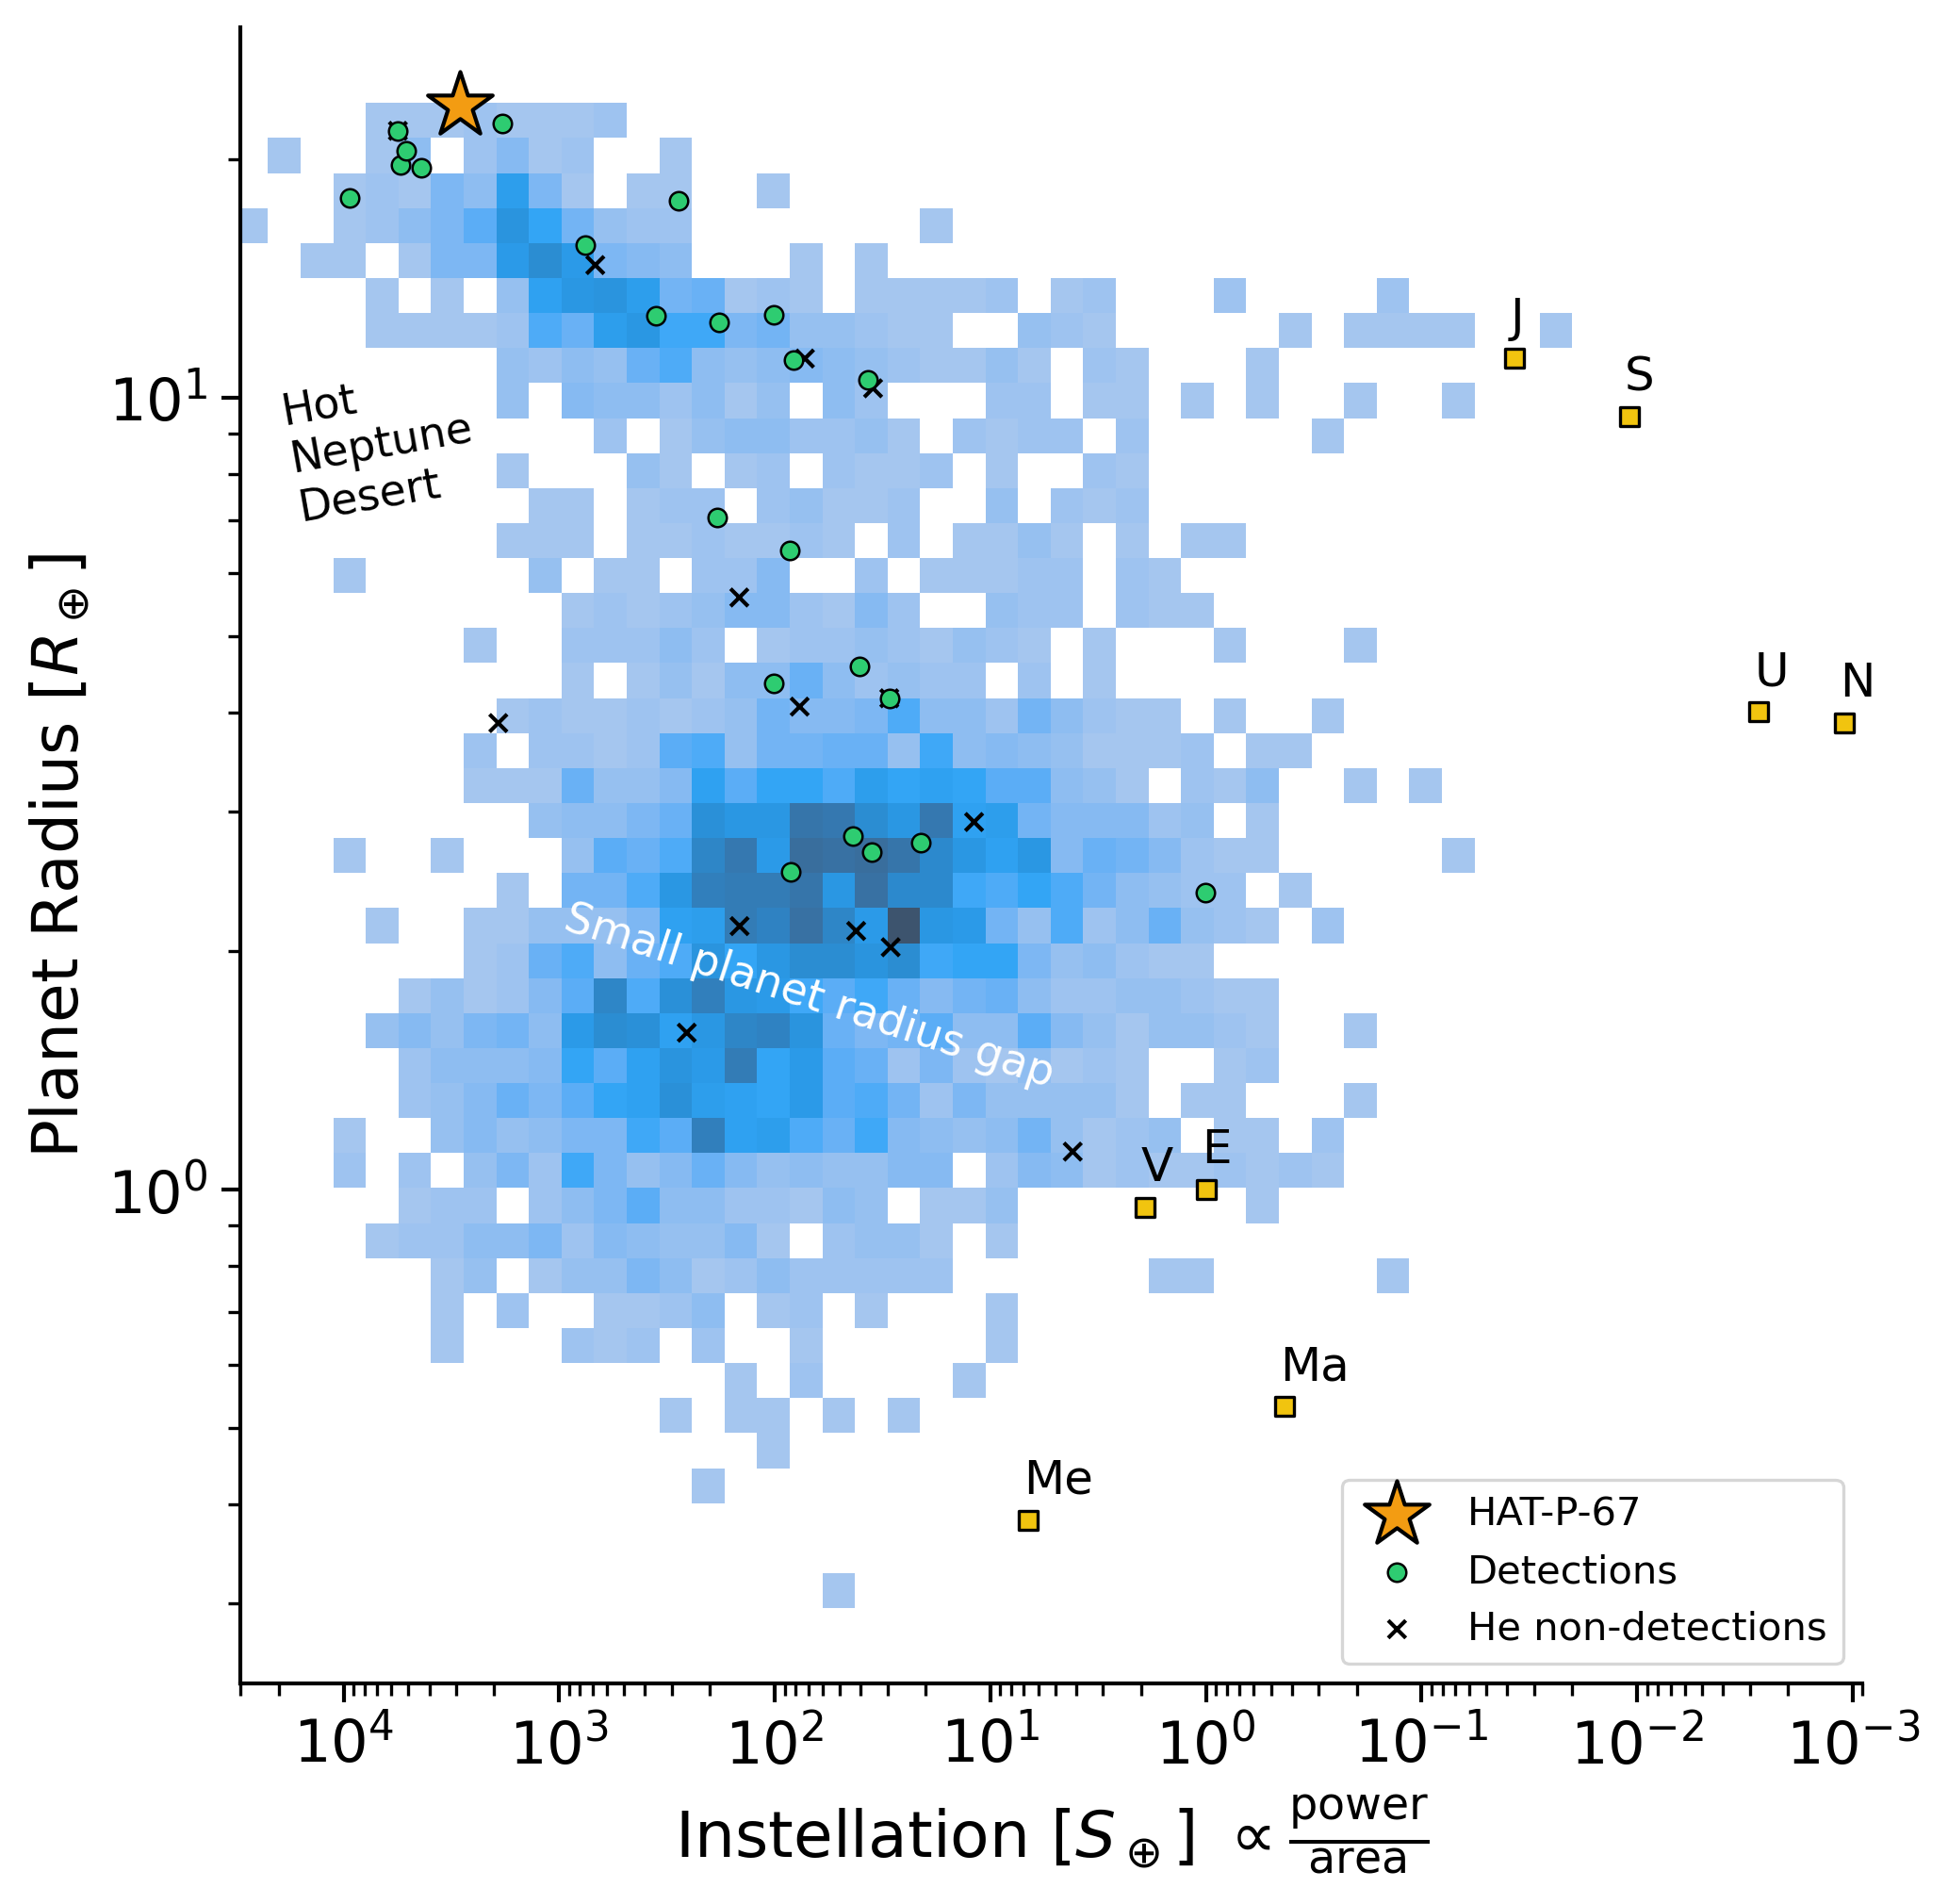
\includegraphics[width=\linewidth]{figures/HAT-P-67b_radius_valley.png}
    \caption{Overview of exoplanet size versus instellation.  Inflated Hot Jupiters appear as the cluster of sources larger than Jupiter and receiving up to 100 to 10,000 $\times$ as much insolation.  The pixel bins reflect the observed density of over 5000 planets accessed from the NASA Exoplanet Archive.  The star symbol shows the inflated position of \hatpb.}
    \label{fig:instellation}
\end{figure}

Here we present a multi-year observational campaign searching for atmospheric escape in \object{HAT-P-67 b}, an inflated hot Saturn orbiting an F type sub-giant at an orbital separation of 0.06 AU \citep{2017AJ....153..211Z}.  The strong insolation combined with \object{HAT-P-67 b}'s low surface gravity makes it an excellent candidate for strong atmospheric mass loss.  It orbits an evolved star, opening the prospect for ``re-inflation'' as the planet's insolation increased over time with the star's expansion.  Its status as a rare inflated Hot Saturn make \object{HAT-P-67 b} a promising laboratory, including but not limited to, testing the inflationary predictions of the Ohmic dissipation mechanism.


\section{Observations}
\subsection{Habitable Zone Planet Finder (HPF)}

The Habitable Zone Planet Finder Spectrograph \citep[HPF;][]{2012SPIE.8446E..1SM,2014SPIE.9147E..1GM, 2019Optic...6..233M} on the queue-scheduled 10-meter \emph{Hobby-Eberly Telescope} \citep[HET;][]{1998SPIE.3352...34R} operates in the near-IR from $8100-12800~$\AA~ spanning the \textit{z}, \textit{Y}, and \textit{J} bands at spectral resolving power $R=55,000$. The HET fixed-elevation design \citep{2007PASP..119..556S} limits the observability of \object{HAT-P-67} to less than 1 hour ``tracks'' for a fixed range of hour angles before (east track) and after (west track) the star transits the meridian.  Whereas conventional steerable telescopes could conduct continuous point-and-stare observations of \object{HAT-P-67} for hours, HET cannot.  In practice, this limitation means that in-transit and out-of-transit observational phases were rarely possible on the same night.  Instead, we organized the observations into four campaigns to coincide with \object{HAT-P-67 b} transits on the nights beginning 2020 April 28, 2020 May 22, 2020 June 15, and 2022 April 28.  These campaigns have out-of-transit observations at least one night before and one night after, and often two nights on either side of the transit.  Two more transits were obtained in 2022 June-July without the visits immediately before and after.  The in-transit nights had up to 14 exposures per HET track, with integration times between 5-8.5 minutes.  We also obtained random-in-phase low priority ``P4'' queue-filler observations.  These out-of-transit snapshot observations typically received 4 or fewer individual exposures.  We observed HAT-P-67 with HPF for a total 41 visits on 39 unique nights, with two of those nights observing both an east and a west HET track.  The total on-source integration time exceeds 13.8 hours.  Table \ref{tabHPFLog} summarizes the log of observations.

The observation scheduling was strategically restricted to the spring season when the Barycentric Earth Radial Velocity (BERV) would Doppler shift telluric absorption lines sufficiently far away from the core of the Helium 10833$\AA~$ feature.  The small BERV still means the redward Helium linewing has significant telluric contamination between 10834-10836 \AA, but the core and blue line wings appear relatively pristine.

Only 19 out of the 39 nights possess A0V telluric calibration standard stars.  These standard stars, when available, were used to spot-check our telluric mitigation strategy.


\begin{deluxetable}{lccrchr}
    \tablewidth{0pc}
    \tabletypesize{\scriptsize}
    \tablecaption{
        HPF Observation Log
        \label{tabHPFLog}
    }
    \tablehead{
        \colhead{Date}   &
        \colhead{Track} &
        \colhead{Transit?} &
        \colhead{BTJD} &
        \colhead{$N_\mathrm{exp}$} &
        \nocolhead{$t_\mathrm{exp}$} &
        \colhead{$\phi$}\\
        \colhead{}   &
        \colhead{} &
        \colhead{} &
        \colhead{(days)} &
        \colhead{} &
        \nocolhead{(s)} &
        \colhead{$\in(-0.5, 0.5)$}
    }
    \startdata
    2020-04-26 &  east &                 & 1966.78 &             4 & 308.85 &            -0.192 \\
2020-04-27 &  east &      in transit & 1967.79 &            12 & 308.85 &             0.018 \\
2020-04-28 &  east &                 & 1968.78 &             4 & 308.85 &             0.225 \\
2020-05-19 &  west &                 & 1989.95 &             4 & 308.85 &            -0.373 \\
2020-05-20 &  west &                 & 1990.94 &             4 & 308.85 &            -0.169 \\
2020-05-21 &  east &      in transit & 1991.72 &            14 & 308.85 &            -0.006 \\
2020-05-22 &  west &                 & 1992.93 &             4 & 308.85 &             0.246 \\
2020-05-23 &  west &                 & 1993.94 &             4 & 308.85 &             0.455 \\
2020-06-12 &  west &                 & 2013.89 &             3 & 308.85 &            -0.397 \\
2020-06-13 &  west &                 & 2014.89 &             4 & 308.85 &            -0.190 \\
2020-06-14 &  east &                 & 2015.64 &             6 & 308.85 &            -0.032 \\
2020-06-14 &  east &      in transit & 2015.66 &             3 & 308.85 &            -0.029 \\
2020-06-14 &  west &      in transit & 2015.89 &             9 & 308.85 &             0.019 \\
2020-06-15 &  west &                 & 2016.87 &             4 & 308.85 &             0.224 \\
2020-06-17 &  west &                 & 2018.88 &             4 & 308.85 &            -0.360 \\
2020-07-21 &  west &                 & 2052.79 &             2 & 511.20 &            -0.309 \\
2020-07-31 &  west &                 & 2062.75 &             2 & 511.20 &            -0.240 \\
2021-01-30 &  east &                 & 2246.03 &             2 & 511.20 &            -0.136 \\
2021-01-31 &  east &                 & 2247.02 &             2 & 511.20 &             0.070 \\
2021-02-23 &  east &                 & 2269.96 &             1 & 511.20 &            -0.161 \\
2021-02-25 &  east &                 & 2271.94 &             2 & 511.20 &             0.250 \\
2021-03-03 &  east &                 & 2277.93 &             2 & 511.20 &             0.496 \\
2021-03-30 &  east &                 & 2304.86 &             2 & 511.20 &             0.094 \\
2022-04-27 &  east &                 & 2697.79 &             4 & 308.85 &            -0.217 \\
2022-04-28 &  east &      in transit & 2698.78 &            14 & 308.85 &            -0.011 \\
2022-04-29 &  east &                 & 2699.77 &             4 & 308.85 &             0.196 \\
2022-04-30 &  east &                 & 2700.77 &             4 & 308.85 &             0.403 \\
2022-05-01 &  east &                 & 2701.77 &             4 & 308.85 &            -0.390 \\
2022-06-19 &  east &                 & 2750.64 &             3 & 308.85 &            -0.230 \\
2022-06-21 &  east &                 & 2752.64 &             3 & 308.85 &             0.187 \\
2022-06-21 &  west &                 & 2752.86 &             3 & 308.85 &             0.232 \\
2022-06-22 &  west &                 & 2753.86 &             3 & 308.85 &             0.439 \\
2022-06-25 &  east &      in transit & 2756.64 &             1 & 308.85 &             0.017 \\
2022-06-30 &  west &                 & 2761.85 &             1 & 308.85 &             0.101 \\
2022-07-09 &  west &                 & 2770.82 &             1 & 308.85 &            -0.035 \\
2022-07-10 &  west &                 & 2771.81 &             1 & 308.85 &             0.172 \\
2022-07-12 &  west &                 & 2773.82 &             3 & 308.85 &            -0.411 \\
2022-07-14 &  west &      in transit & 2775.78 &             1 & 308.85 &            -0.003 \\
2022-07-15 &  west &                 & 2776.80 &             1 & 308.85 &             0.209 \\
2022-07-19 &  west &                 & 2780.77 &             1 & 308.85 &             0.034 \\
2022-07-28 &  west &                 & 2789.74 &             1 & 308.85 &            -0.101 \\
2022-07-29 &  west &                 & 2790.78 &             1 & 308.85 &             0.115 \\
    \enddata
    \tablecomments{All exposure times were 308.85~s except for observations from 2020-07-21 to 2021-03-30, which were 511.20~s.}
\end{deluxetable}

\subsection{TESS Light Curves}
HAT-P-67 was observed with the \emph{Transiting Exoplanet Survey Satellite} \citep[TESS,][]{2014SPIE.9143E..20R} in Sectors 24, 26, 51, 52, 53 with 2-minute cadence, and in Sector 25 with 30-minute (FFI) cadence.  The Sector 25 FFI data appeared malformed, possibly due to problems with pipeline CCD smear correction, and was disregarded.

We also assembled a comparison sample of about 1000 lightcurves to interpret the  prevalence of lightcurve modulation and stellar activity among broadly F subgiant-like stars.  We selected sources based on \emph{Gaia} DR3 $T_\mathrm{eff}$ estimates and similar $\log{g}$,  and availability of at least one sector of TESS 2-minute cadence data.  We also visually spot-checked these lightcurves to understand artifacts and windowing effects.

\subsection{ASAS-SN}
We retrieved ground-based photometry with the \emph{All-Sky Automated Survey for Supernovae} (ASAS-SN) using the Sky-Portal \citep{shappee14,2017PASP..129j4502K}.  The precision of ASAS-SN was too low to perceive stellar variability, and so we can place a relatively uninformative limit of $<5\%$ stellar variability on years-long timescales.

\subsection{DASCH}
\hatp appears in the Harvard Plate Archive, with 5809 measurements digitized through DASCH, spanning over 120 years of coarse photometric monitoring.  In principle these datasets could inform long-term variability trends such as stellar cycles.  In practice the 0.15 magnitude jitter appears too coarse to perceive any genuine astrophysical variability, with no conspicuous trend seen.  We can therefore place a relatively mild constraint that the star is stable at the $\sim30\%$ level over periods of tens to hundreds of years.

\subsection{Gaia DR3}\label{gaiadr3}
The stellar system consists of a binary with an M dwarf companion HAT-P-67B (\emph{Gaia DR3 1358614983131339904}) separated on-sky by $9\farcs0$ \citep{2019MNRAS.490.5088M}.  HAT-P-67A (\emph{Gaia DR3 1358614983131339392}) has a parallax of $2.69\pm0.01$ mas in \emph{Gaia} DR3, placing it at about 372$\pm$1.4 pc.  Minor corrections to the parallax uncertainty \citep{2021MNRAS.506.2269E} and bias \citep{2021A&A...649A...4L} appear negligible for the $G=9.98$ source.  The DR3 parallax places the system about 8.7\% farther than previously estimated by \citet{2017AJ....153..211Z}, which adopted a \emph{Gaia} DR1-informed parallax of $2.92\pm0.23$ mas, including a $-0.325$ mas bias term from \citep{2016ApJ...831L...6S}.  Its coarse \emph{Gaia}-based estimates for RV and Doppler broadening are consistent with the more precise values published in \citet{2017AJ....153..211Z}.  Its wide companion HAT-P-67B  \citep{2019MNRAS.490.5088M} has nearly identical parallax ($2.58\pm0.05$ mas) and proper motions, confirming its interpretation as co-moving, with projected separation of about 3400 AU.  The IAU naming convention would demand HAT-P-67A\emph{b} to refer to the planet.  Hereafter, we simply drop the A designation for notational simplicity, since the wide companion will not factor into our analysis.

\subsection{Other archives}
\hatp has one $R\sim8000$ spectrum from the Intermediate Dispersion Spectrograph on the INT, centered near 4000 \AA.  It has 26 photometry points from \emph{Pan-STARRS} spread across its 5 filters.  The other archival observations have been previously reported by \citet{2017AJ....153..211Z}, including Keck HIRES, Keck NIRC2, and WIYN High-Resolution Infrared Camera.  The northern source does not appear in ESO archives, nor the Gemini Archive, and it is not publicly accessible in the Zwicky Transient Factory (ZTF) archive.  It was not targeted by \emph{Spitzer} or \emph{Hubble}.

\begin{figure*}
    \centering
    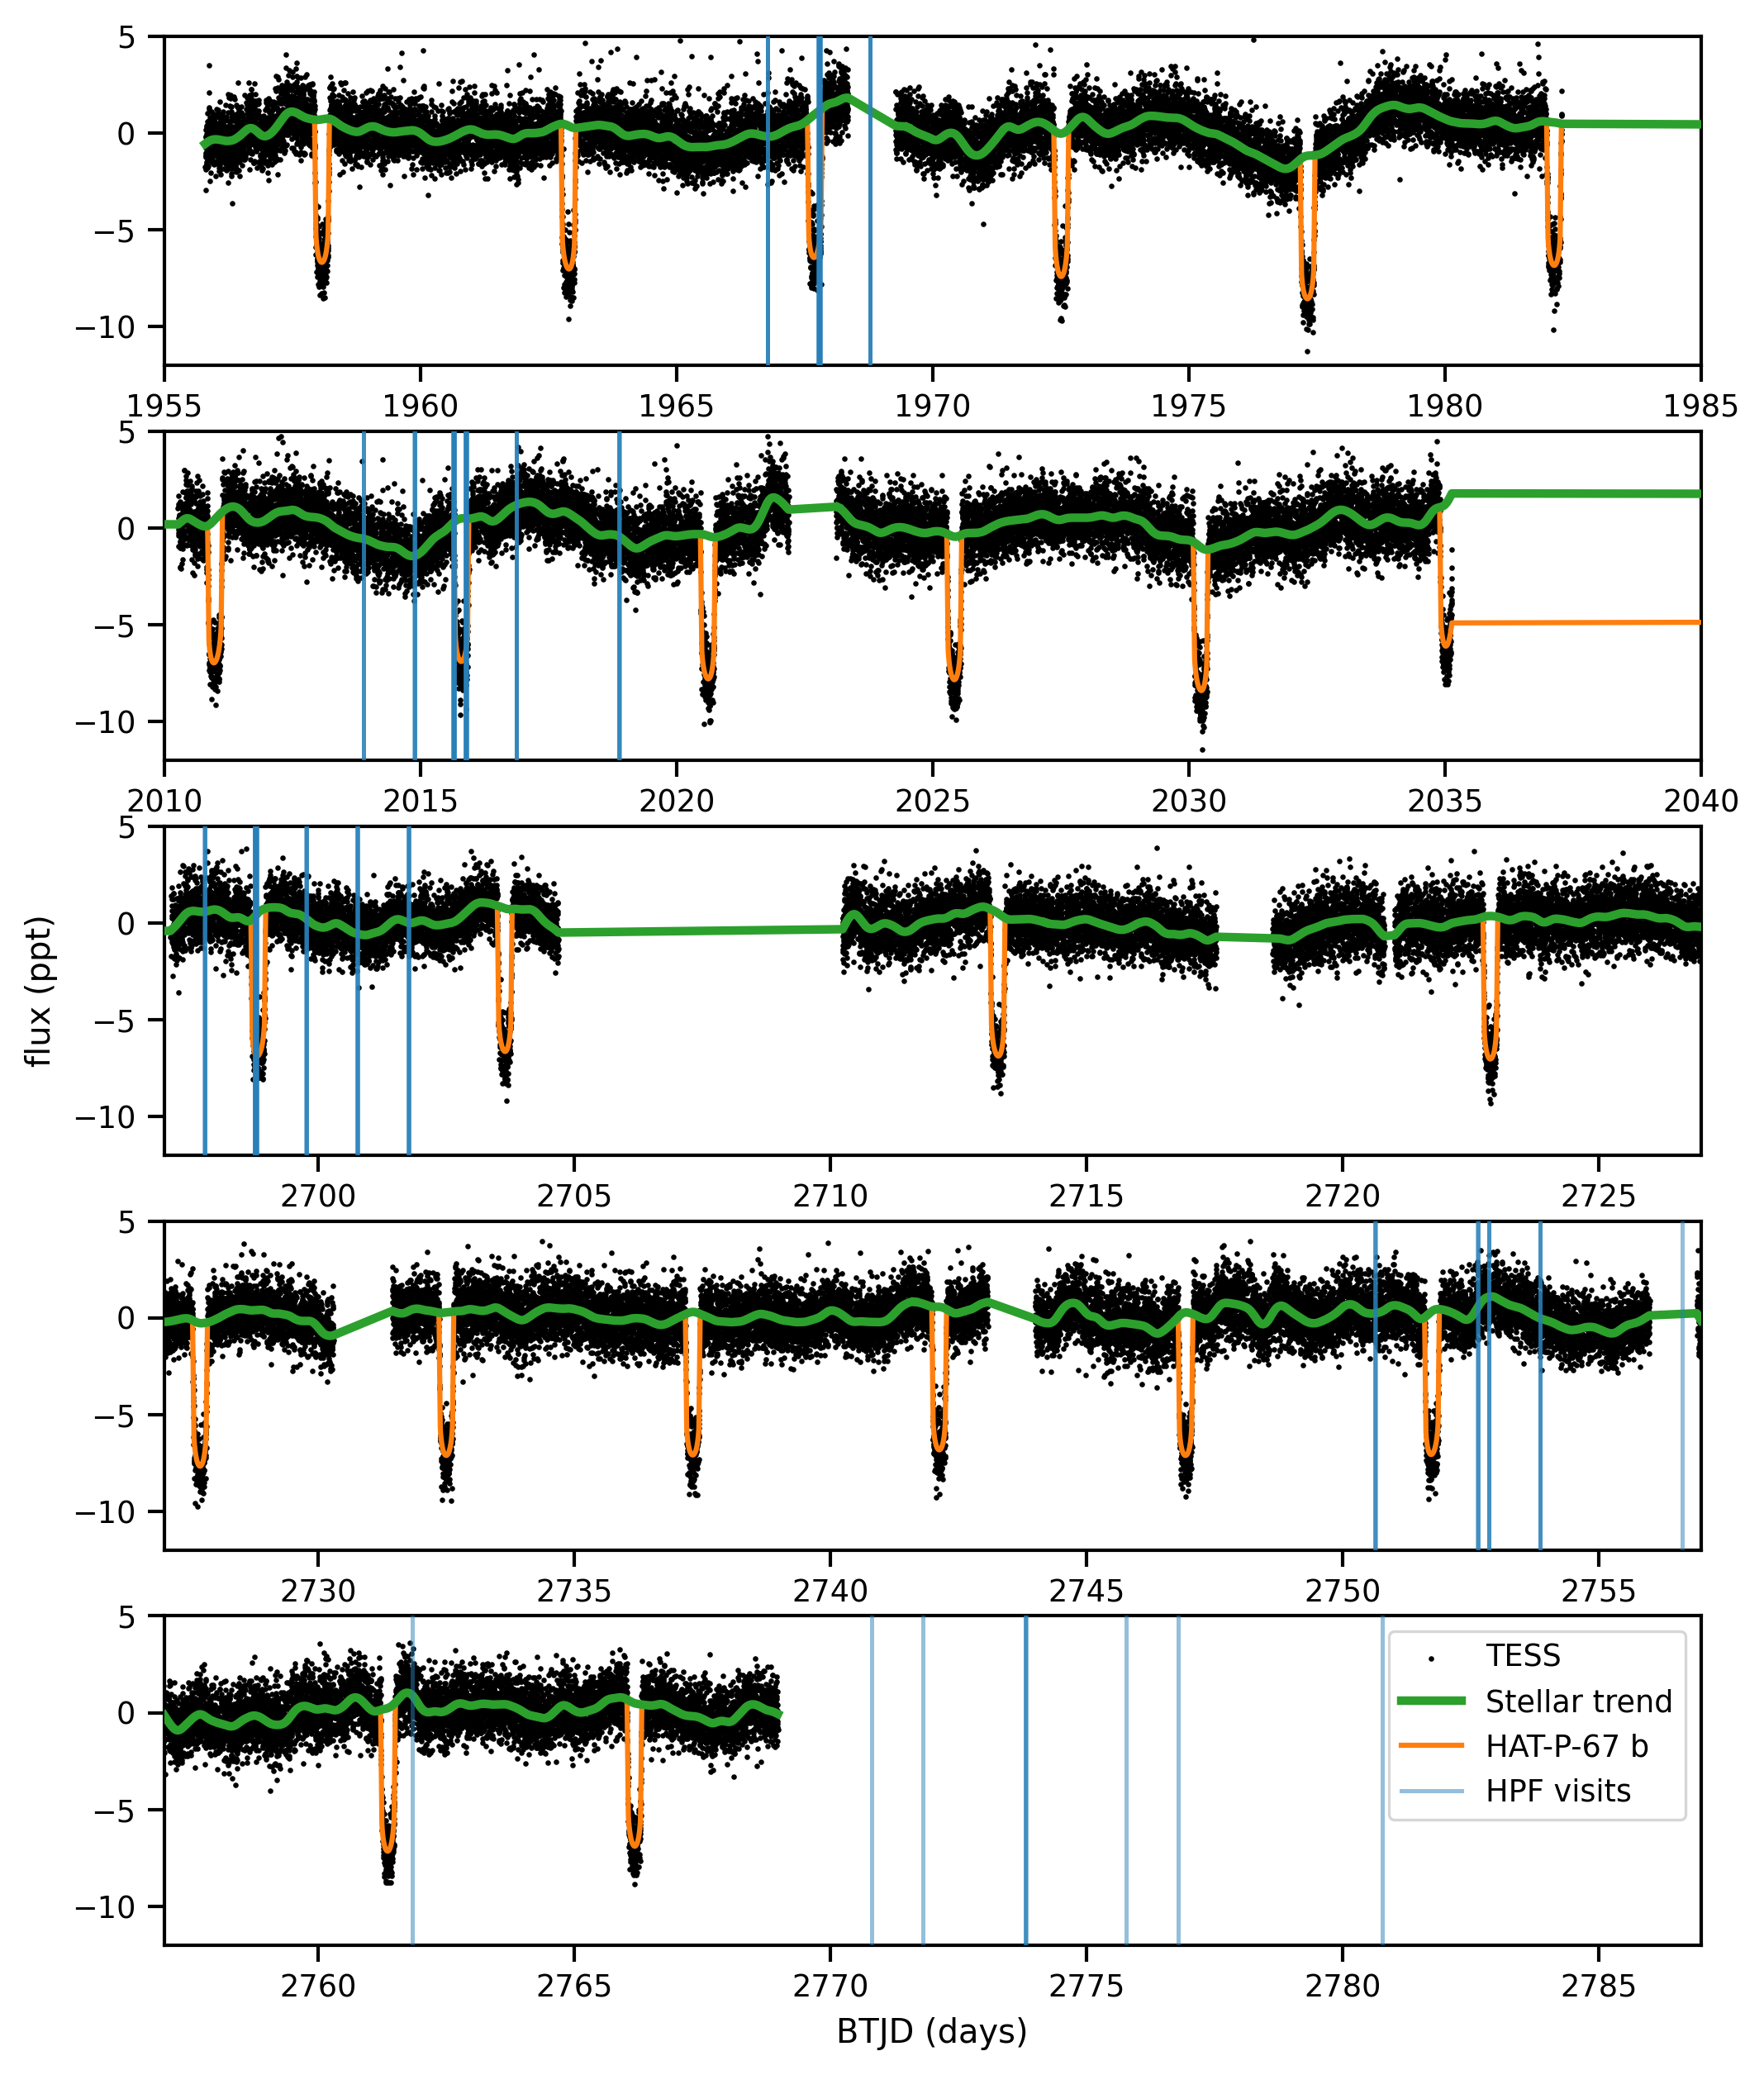
\includegraphics[width=0.7\linewidth]{figures/TESS_HAT-P-67b_overview.png}
    \caption{Overview of all available TESS Sectors showing 24 full or partial transits with 34 visits with HPF (vertical gray bars), 7 of which coincide with transits, and the rest sample out-of-transit phase.  The 8 HPF visits between BTJD 2050 and 2690 are not shown.}
    \label{fig:TESSoverview}
\end{figure*}


\section{Analysis}

\subsection{Gaia DR3}
\citet{2017AJ....153..211Z} previously derived stellar radius estimates of 2.1-2.7 $R_\odot$ through Spectral Energy Distribution (SED) isochrone fitting as part of a joint orbit fit.  We systematically increase those stellar radius estimates by 8.7\% to match the greater Gaia \emph{DR3} distance (\S \ref{gaiadr3}).  For a fixed $R_p/R_\star$, the larger $R_\star$ implies a proportionally larger planet radius. This update systematically decreases the estimate for the already-low density of HAT-P-67 by 28\%, to a mere 0.035 g$\;$cm$^{-3}$, albeit with significant uncertainties from the weak mass constraint, and from the model dependence of multiple orbit fits.

\subsection{TESS Light Curve}
Previously, \hatp transits had only been detected with \emph{HATNet} \citep{2004PASP..116..266B} and followed up with KeplerCam on the FLWO 1.2 m telescope \citep{2017AJ....153..211Z}. These ground-based photometers were not intended to measure long term stellar variability signals.  We therefore examined the \emph{TESS} lightcurves for out-of-transit photometric variability.  The revised precision and continuous coverage of \emph{TESS} can refine the orbital solution.

\subsubsection{Revised exoplanet orbital parameters}
We assembled a composite lightcurve by stitching TESS Sectors 24, 26, 51, 52, 53, which were reduced with the default SPOC pipeline \citep{2020RNAAS...4..201C}, and lightly post-processed with \texttt{lightkurve} \citep{geert_barentsen_2019_2565212}.  These TESS data exhibit an RMS scatter of better than 1 part-per-thousand (ppt) at native 2-minute sampling.  We fit a Keplerian orbit model to the TESS lightcurve using the \texttt{exoplanet} framework \citep{exoplanet:joss}.  We obtained a best fit orbital period of $4.81011$ days, non-zero eccentricity of 0.19, an impact parameter of 0.46, planet-to-star radius ratio of 0.0823, transit depth of 0.74\%, and $T_0$ of 1958.07933 in BTJD.  These properties are consistent with the previously reported values from \citet{2017AJ....153..211Z} and the updated ephemeris of \citet{2022ApJS..259...62I}.  Figure \ref{fig:TESSoverview} shows an overview of all the TESS Sectors demarcated with the epochs of HPF measurements.  Figure \ref{fig:transit} shows the best-fit orbit overlaid on the detrended TESS lightcurve.  Table \ref{tabOrbit} lists one of the previous orbit determinations and solution reported here.

\subsubsection{Stellar rotation rate from periodogram analysis}

The TESS Sector 26 lightcurve exhibits a weak $\sim$3 ppt peak-to-valley out-of-transit modulation on timescales comparable to the exoplanet orbit. TESS Sectors 51-53 do not show as conspicuous a modulation signal.  Figure \ref{fig:TESSoverview} shows this modulation in the minimally processed TESS lightcurve.  We fit the TESS lightcurve modulation with a quasiperiodic Gaussian Process (GP) model using \texttt{celerite} \citep{celerite1,celerite2}.  The GP model fit to the entire composite lightcurve yields a period of 4.7 days; when fit to individual sectors alone the periods hover around 5.9 days.

If we attribute this TESS modulation signal to stellar activity, we obtain a rotation period $P_\mathrm{rot}$ between 4.7 and 5.9 days.  We can constrain the expected rotation period based on our revised stellar radius estimate, stellar rotation rate from $v\sin{i}$, and the observation of $i\sim90^\circ$ from orbit fitting and Doppler tomography \citep{2017AJ....153..211Z}.  We adopt a high limit of $v\sin{i}=35.8\pm1.1$ km/s and a lower $v\sin{i}=30.9\pm2$ km/s value if macroturbulence is accounted for.  We obtain a range of $3.2 < P_\mathrm{rot}  < 4.8 $ days.  This range may be typical for F stars that have not yet evolved too far into the sub-giant branch \citep{2022ApJ...930....7A}.  The geometrical constraint includes the 4.7 day GP-based modulation period derived from the stitched TESS lightcurve, but is lower than the 5.9 day per-Sector fits, slightly preferring the lower 4.7 day modulation as the stellar rotation period.  The 5.9 day value would require a stellar radius over 3.2$R_\odot$, which appears consistent with only an eccentric orbit model combined with the Geneva isochrone \citep{2017AJ....153..211Z}.


\begin{figure}
    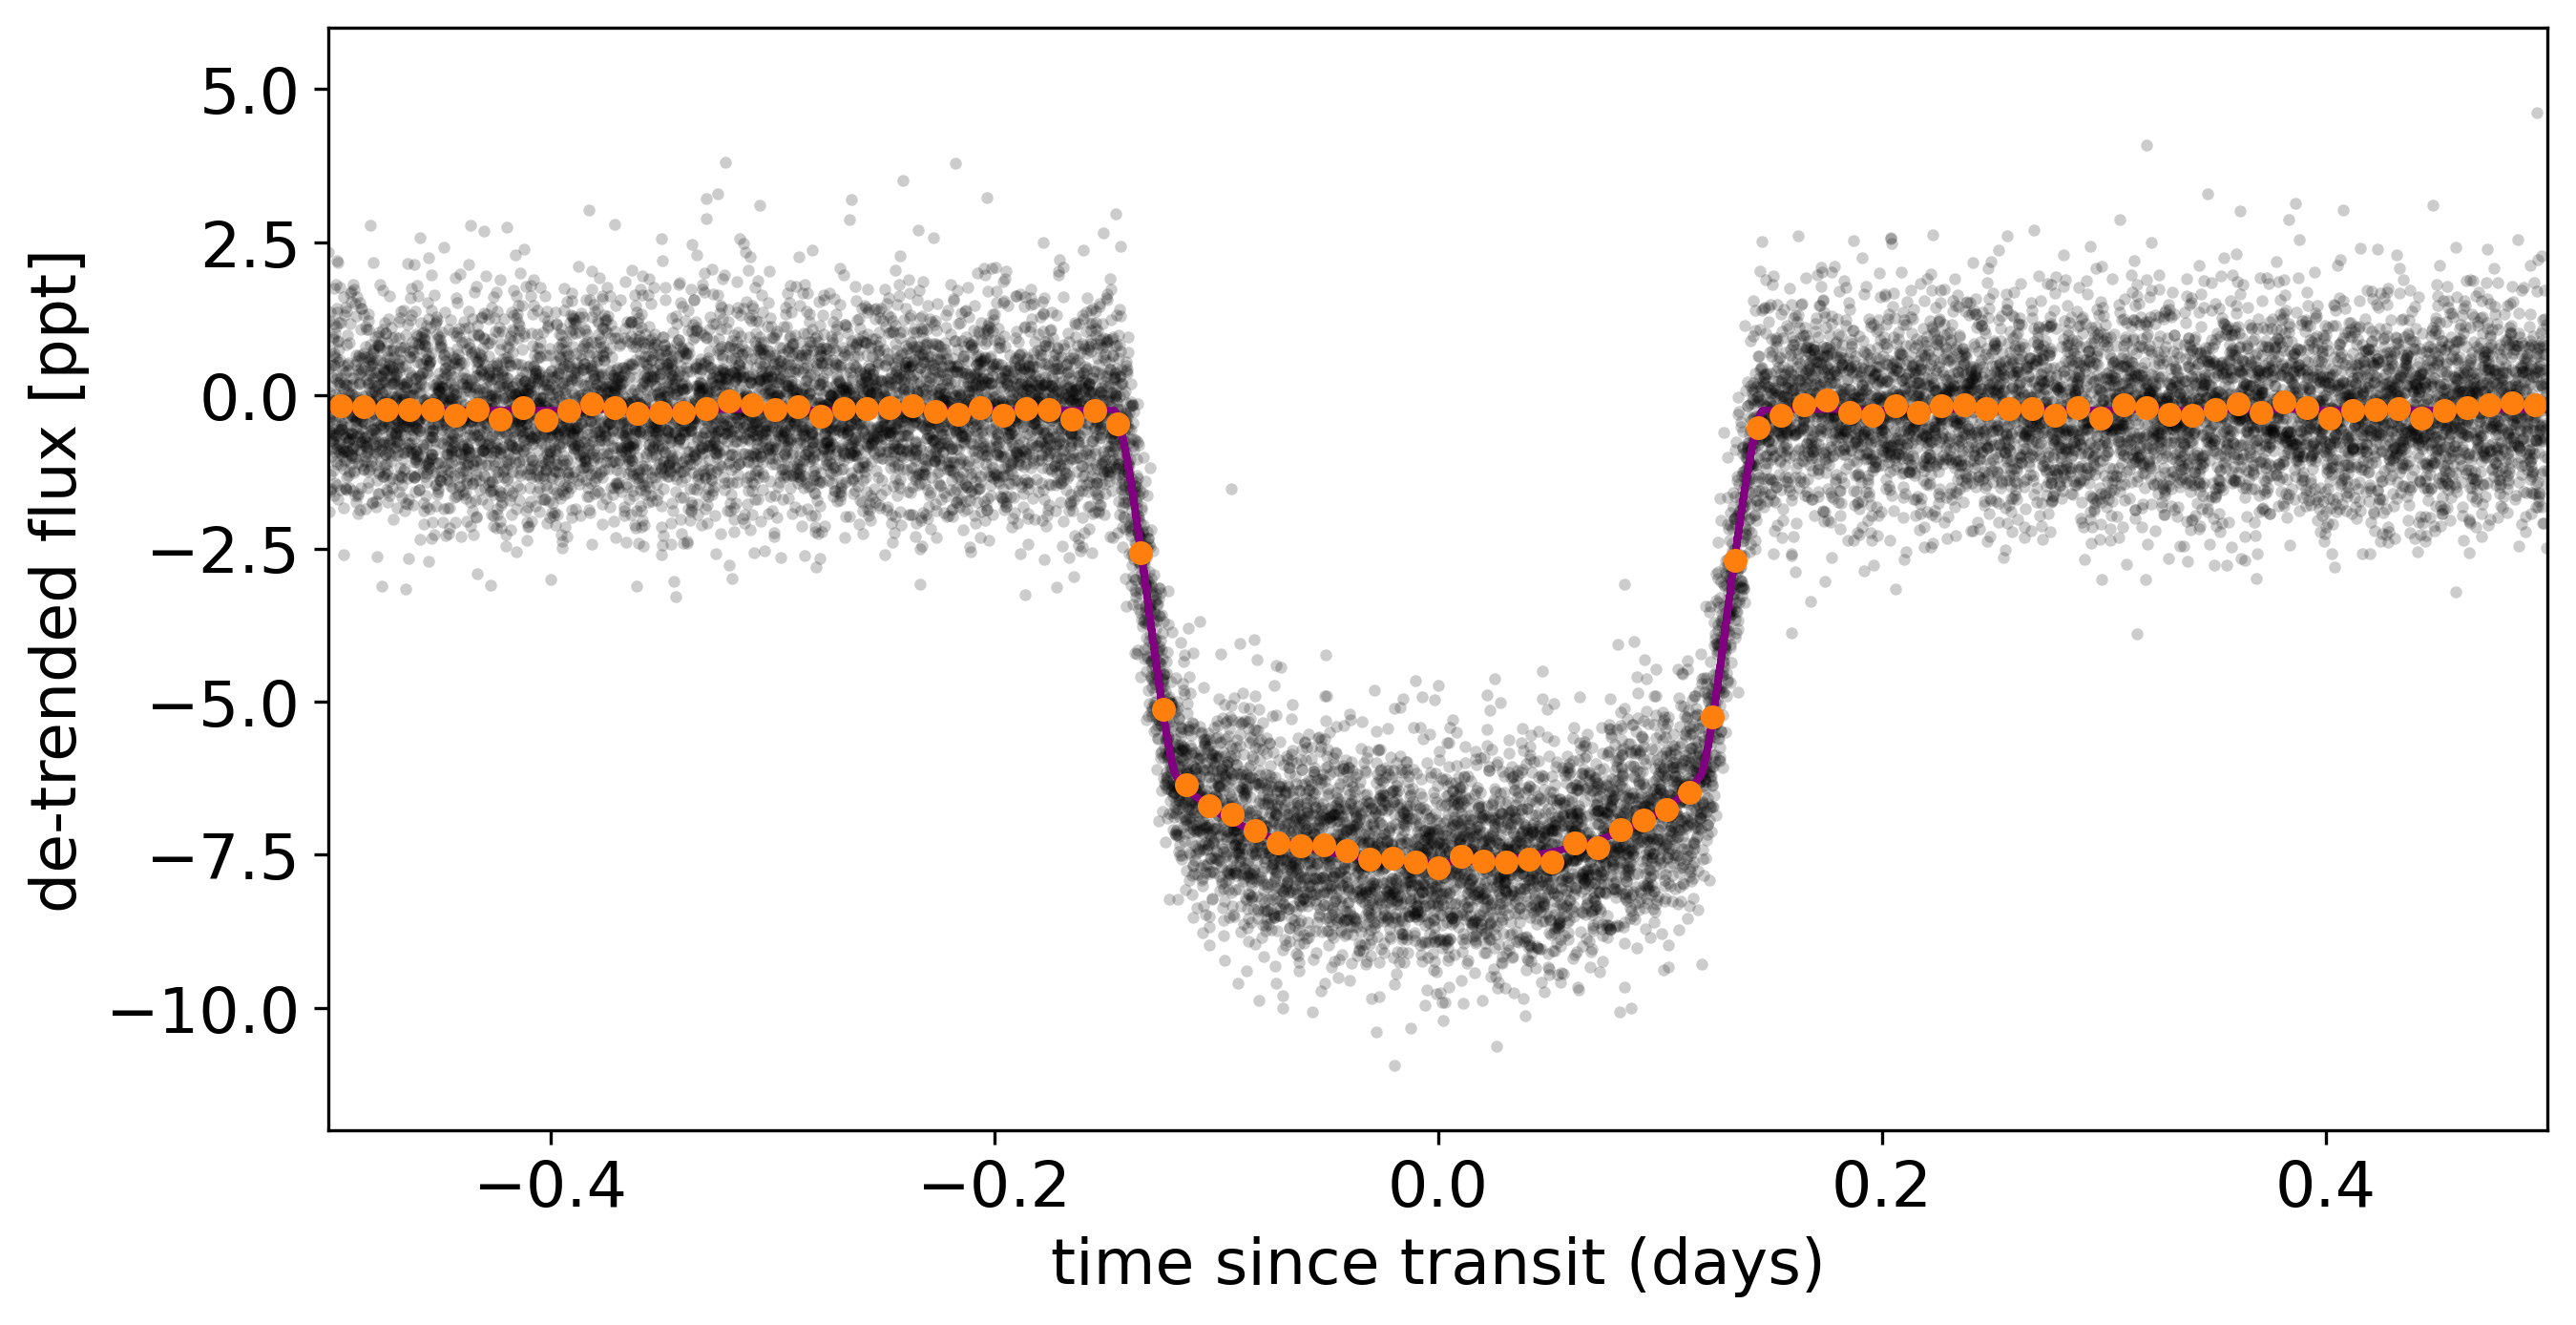
\includegraphics[width=\linewidth]{figures/best_fit_orbit.png}
    \caption{Best fit orbit overlaid on the composite TESS lightcurve.}
    \label{fig:transit}
\end{figure}

\subsubsection{Lightcurve modulation amplitude}
We computed the peak-to-valley modulation for the 1000-source \emph{TESS} comparison sample, defined as the difference between the 90$^{th}$ to 10$^{th}$ percentile of each normalized \emph{TESS} lightcurve.  Most lightcurves appear consistent with negligible astrophysical variability and/or variability predominated by instrumental artifacts. \object{HAT-P-67}'s 0.36$\%$ lightcurve modulation ranked in the 87$^{th}$ percentile of the ensemble, about 0.5$\times$ above the median.  Sources more variable than HAT-P-67 exhibited 3-5$\times$ its amplitude of modulation.


\begin{deluxetable*}{lrrrh}
    \tablewidth{0pc}
    \tabletypesize{\scriptsize}
    \tablecaption{
        Revised orbital and planetary parameters
        \label{tabOrbit}
    }
    \tablehead{
        \colhead{Parameter}   &
        \colhead{Zhou et al. 2017} &
        \colhead{Ivshina \& Winn 2022} &
        \colhead{This Work} &
        \nocolhead{Alternate}
    }
    \startdata
    %%
    ~~~$P$ (days)             \dotfill    & $4.8101025_{-3.3\times 10^{-7}}^{+4.3\times 10^{-7}}$ & 4.8101046$\pm1.7\times10^{-6}$ & 4.81011 & z \\
    ~~~$T_c$ (${\rm BTJD}$)  \dotfill    & $-1038.61533_{-0.00064}^{+0.00076}$ & 1958.08059$\pm$0.00032 & 1958.07933 & z \\
    ~~~$T_{14}$ (hours)  \dotfill    & $6.9888 \pm 0.046$ &  & 7.0636 & z \\
    ~~~$\rpl/\rstar$          \dotfill    & $0.0834\pm0.0017$ &  & 0.08231 & z \\
    ~~~$b \equiv a \cos i/\rstar$
    \dotfill    & $0.12_{-0.08}^{+0.12}$ &  & 0.45616 & z \\
    \enddata
\end{deluxetable*}


\subsection{HPF analysis}
The raw 2D echellograms were reduced with the \texttt{Goldilocks} package\footnote{\url{https://github.com/grzeimann/Goldilocks_Documentation}}, which outputs 1D extracted spectra for the target, and two reference fibers: blank sky and a laser frequency comb \citep[LFC,][]{2019Optic...6..233M}.  The observations were usually acquired with the LFC turned off, so this unilluminated spectrum was discarded.

The sky fiber and target fiber have slightly different throughputs and illumination properties, with the target fiber receiving $93\%$ of the flux of the sky reference fiber on average.  This ratio depends on wavelength and season at the few percent level.  We quantified the wavelength dependence by acquiring calibration observations of blank sky in both the target and sky fiber.  We applied this wavelength-based scale factor to each target spectrum's associated reference sky fiber to achieve near-imperceptible sky-line residuals.  A few lines exhibit residuals which may arise from genuine differences in the local atmospheric conditions between the target and sky fiber.

We masked spectral regions predicted to have significant telluric lines with a template generated by \texttt{telfit} \citep{2014AJ....148...53G}.  We shifted the spectral coordinates to their common barycentric-corrected reference frame \citep{2014PASP..126..838W} as implemented in \texttt{astropy} \citep{2013A&A...558A..33A,2018AJ....156..123A,2022ApJ...935..167A}.  We flattened the spectra to two pre-selected continuum indices highlighted as vertical blue bands in Figure \ref{fig:HPFheliumOverview}.  The sky-subtraction, telluric masking, barycentric correction, flattening, and all of our other standard pre-processing steps were carried out in the open-source Python interface \texttt{muler} \citep{2022JOSS....7.4302G}.

Figure \ref{fig:HPFheliumOverview} shows a zoom-in on the He 10830 region of interest, with all 152 individual exposures overlaid.  We see a variability in the Helium line of up to 10\%, much greater than the $<1\%$ pixel-to-pixel variation.  The feature width spans about 3~\AA.

\begin{figure}
    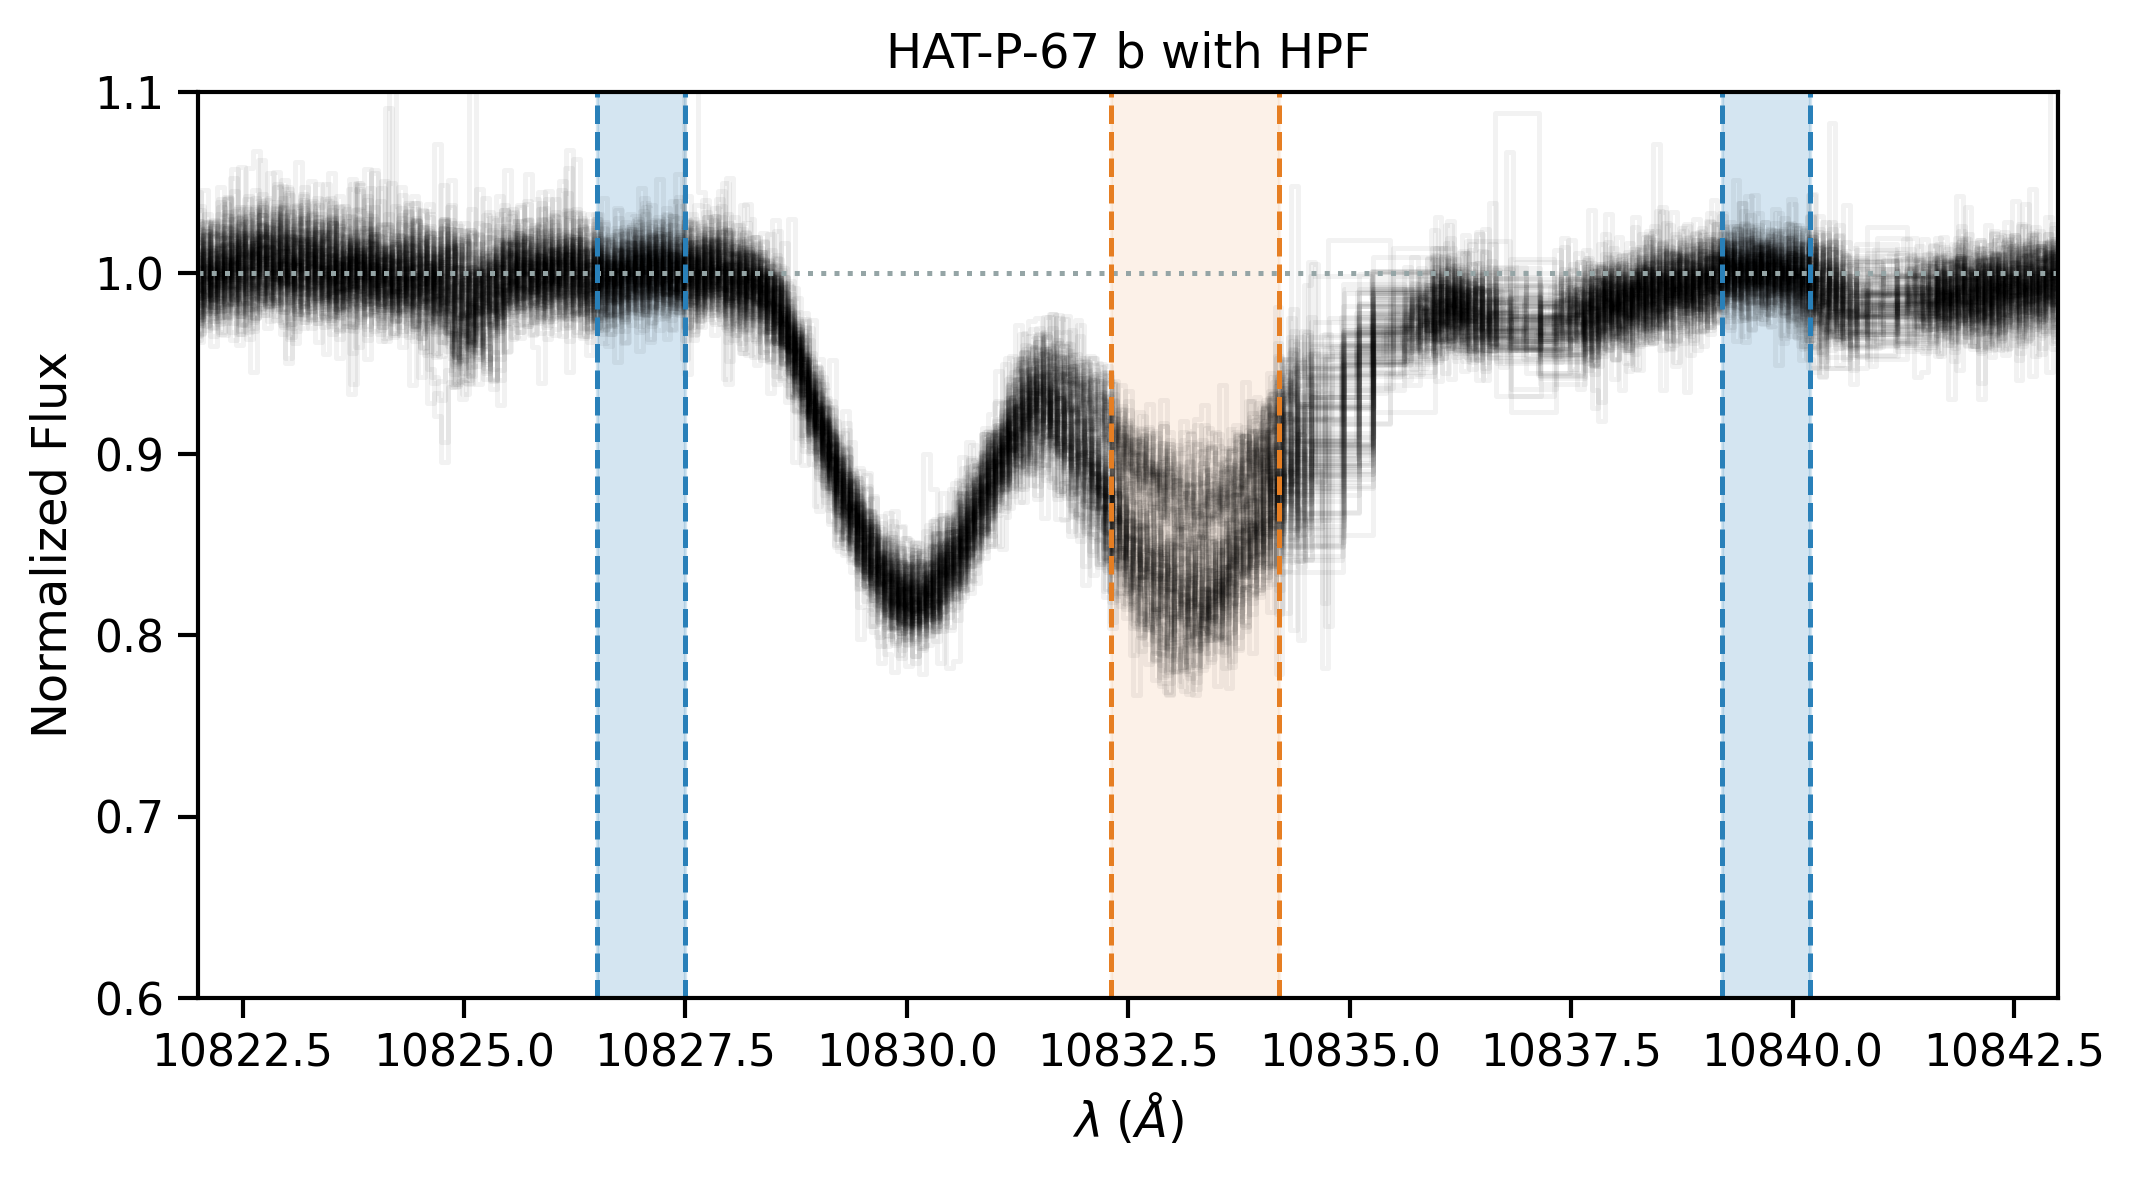
\includegraphics[width=\linewidth]{figures/HAT_P_67b_He_spectrum.png}
    \caption{Overlay of all 128 individual HPF exposures of HAT-P-67, spanning 2020-2022. Variability is seen in the \ion{He}{1} 10833 \AA~ triplet, denoted by the vertical orange shaded band, but not in the adjacent regions.  These snapshot spectra were barycentric corrected, and continuum flattened to the regions in the blue vertical bands.  Sharp telluric absorption lines have been masked in regions near 10835 and 10837.5 $\AA$.}
    \label{fig:HPFheliumOverview}
\end{figure}


The 13.8 hours of exposure, combined with \object{HAT-P-67 b}'s short ($P\sim4.8$ day) period, means that a large fraction of the orbit has been collected, with some phases (especially near transit) heavily sampled, and some other out-of-transit phases sampled more sparsely. For visualization purposes, we constructed a 2-D intensity phase scan, binning in phase and wavelength, and spanning the entire orbit of \object{HAT-P-67 b}.  Figure \ref{fig:HPFscanResid} overlays the planet's approximately $\pm150\;$km/s orbital Doppler velocity, with the stellar rest frame velocity demarcated by the vertical line.  The vanishing $<36$ m/s reflex motion of the star is imperceptible at this scale.  The horizontal dashed lines indicate the moments of transit ingress (-0.03), midcenter (0.0), and egress (+0.03).

The in-transit phases exhibit over 10\% excess absorption peaks.  A large absorption signal can be seen preceding transit ingress, with some significant absorption evident before $-0.2$ in phase.  We construct a fractional residual absorption spectrum by subtracting off and re-normalizing to the non-varying baseline.  We define the non-varying baseline spectrum as the average over phases $0.3-0.5$, which exhibited stable spectra with the least absorption.  Figure \ref{fig:HPFscanResid} shows that significant absorption can be seen as a few percent at $-0.37$ in phase, rising to 10\% just before and during transit.  The egress drop off is extremely sharp, with almost no excess absorption directly after transit.

% Describe construction of residual spectra

We estimated bulk characteristics of the Helium lines by fitting a Gaussian line profile to the 10828$-$10838 \AA~region of the residual spectra.  The single line initialized at 10833 \AA~ was intended to aglomerate all three components of the metastable triplet into a single feature, consistent with their appearance in Figure \ref{fig:HPFheliumOverview}.  The model constructed in this way has a total of 4 parameters: amplitude $A$, location $\lambda_c$, Gaussian width $\sigma$, and constant offset.  We repeated a similar process for the nearby Si line at 10830 \AA~as a control sample.

Excess is confidently detected at \censor{X} phases at \censor{Z}$\sigma$.  The full-width at half maximum (FWHM) of the feature is about 1.8-2.6~\AA, equivalent to a line-of-sight velocity distribution in the range of 50-75~km/s.  Individual fits to the He feature show a typical line center uncertainty $\pm0.1$~\AA~ or better.  The out-of-transit phases exhibit a line center position of 10833.4~\AA, consistent with the stellar \ion{He}{1} rest frame zero velocity.  The excess absorption resides slightly blueward of the stellar zero restframe velocity reference.  As mentioned previously, the telluric masking near 10836 \AA~ censors our view of the existence (or not) of any redshifted lobe in this region.  A more careful treatment of the telluric absorption could rescue some of the data in this region.  The excess detections exhibit a bulk blueshift of up to 30~km/s.

The excess absorption spectrum exhibits an increasing line-of-sight velocity distribution as the planet transits, going from 60~km/s at ingress, up to 100 km/s at egress.

Finally, we detect a much weaker but still significant post-egress blue-shifted absorption.  This lobe appears to decrease linearly in wavelength, corresponding to a characteristic blueshift increasing from near zero at transit midpoint to 80~km/s 12 hours after transit.  It exhibits a slightly lower line-of-sight velocity distribution of 50 km/s, about half of the peak during transit.


\begin{figure}
    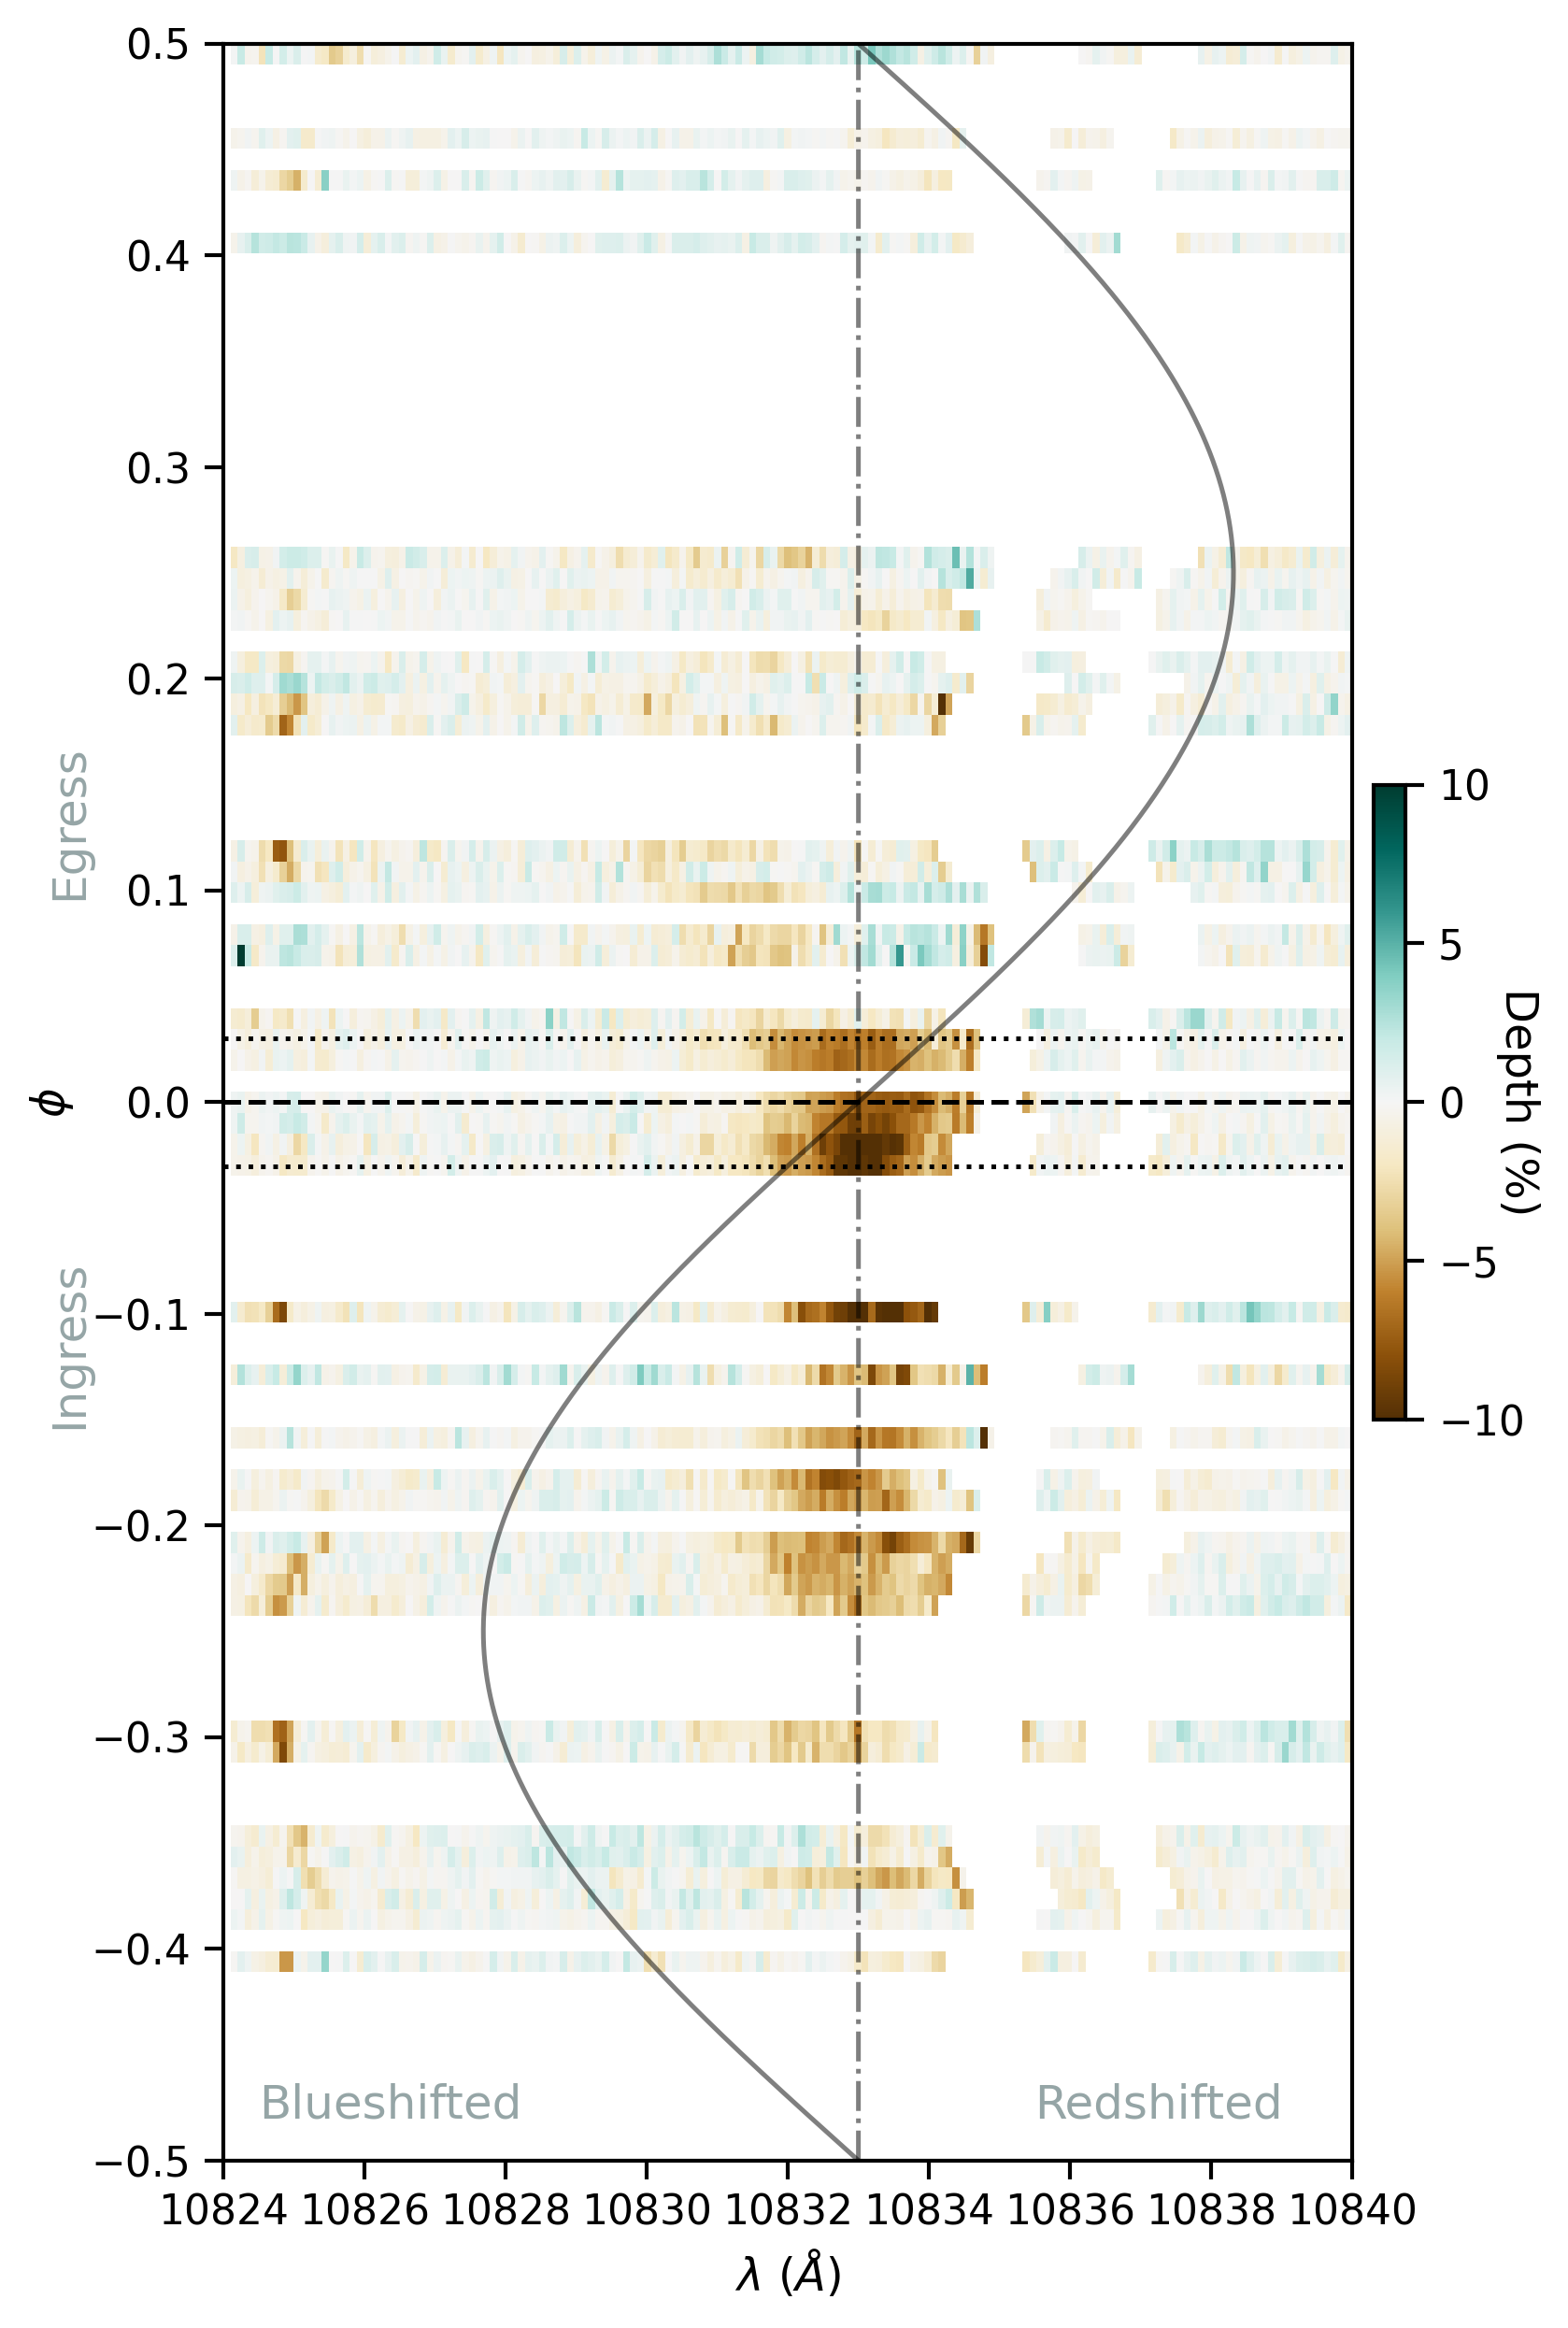
\includegraphics[width=\linewidth]{figures/phase_2D_diagram_resid.png}
    \caption{Absorption depth phase scan over the entire HAT-P-67b orbit from 41 visits with HPF.  }
    \label{fig:HPFscanResid}
\end{figure}


\begin{figure}
    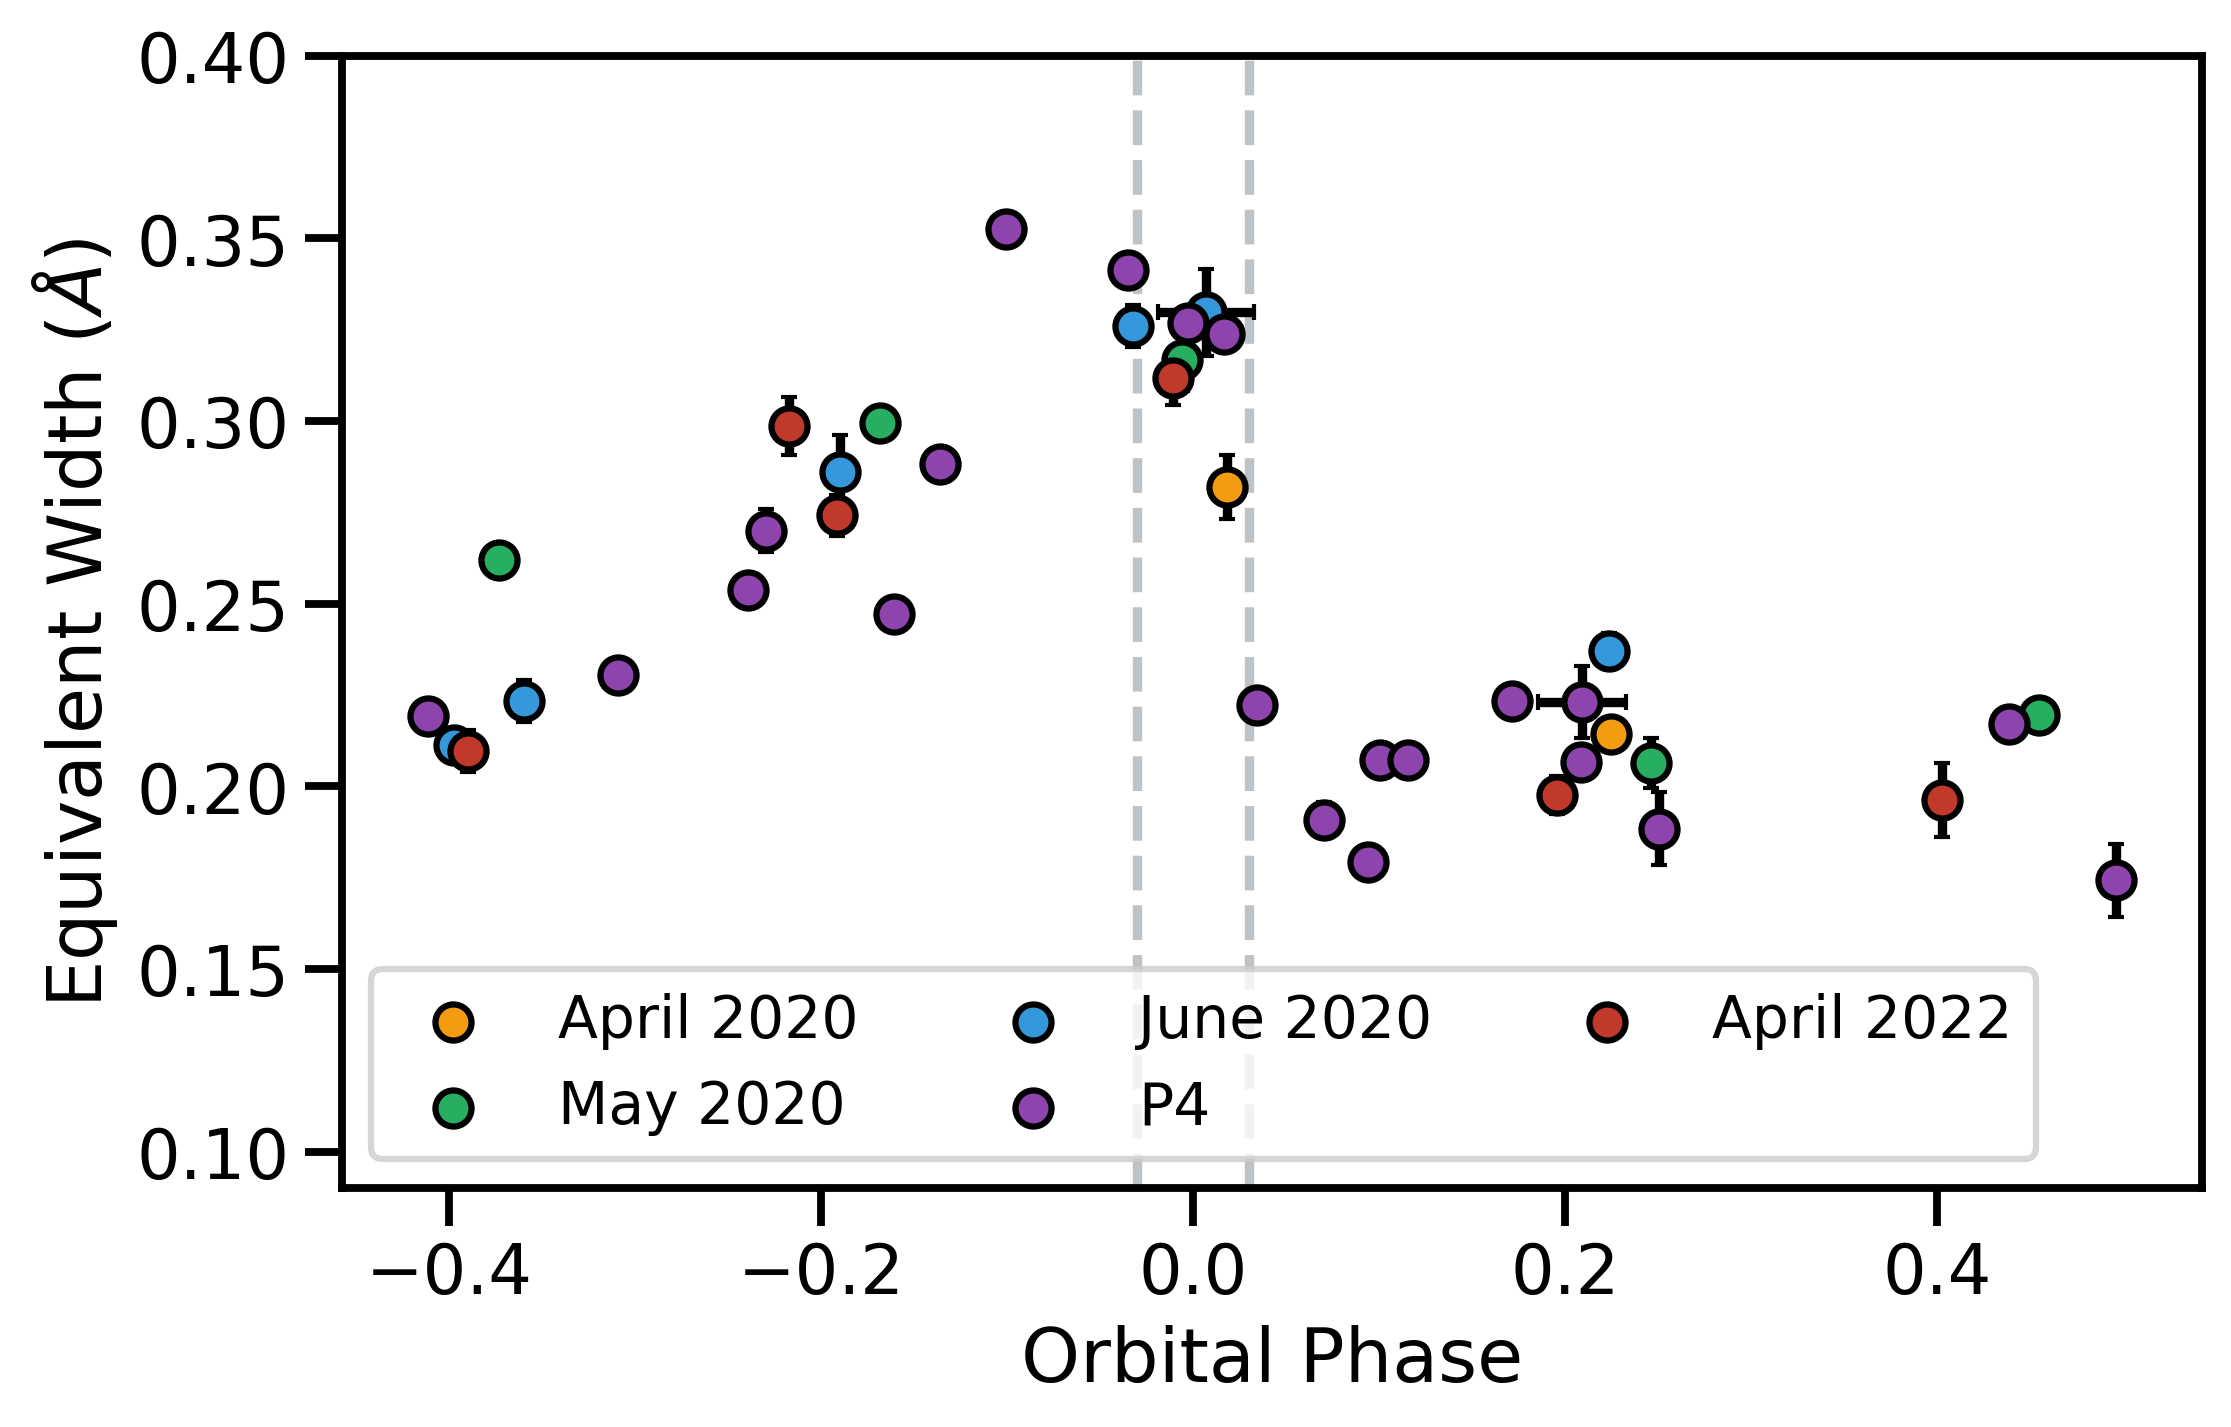
\includegraphics[width=\linewidth]{figures/HAT_P_67b_Helium10830EW_byCampaign.png}
    \caption{Time series EW lightcurve of Helium absorption in HAT-P-67b.  The system exhibits a characteristic absorption leading up to transit, followed by a sharp decline after transit passage.  }
    \label{fig:HPFtimeseries}
\end{figure}

\subsection{Calcium IR Triplet and other line diagnostics}
We examined the \ion{Ca}{2} IR Triplet lines (Ca IRT) for evidence of variability.  No variation was seen in these features, which were pre-processed in the same way as the Helium feature.  Figure \ref{fig:CaPhaseScan} shows a similar phase plot as Figure \ref{fig:HPFscanResid}, adapted to the line at 8662 \AA.  We see no conspicuous variability at this or any of the other Ca IRT lines.  We also found no detectable variability in the Pa$\delta$ line at 10050 \AA, nor other deep lines at 10330 \AA~ and elsewhere.  \ion{He}{1} 10833 appears to be the only conspicuously variable line in the HPF spectrum.

\begin{figure}
    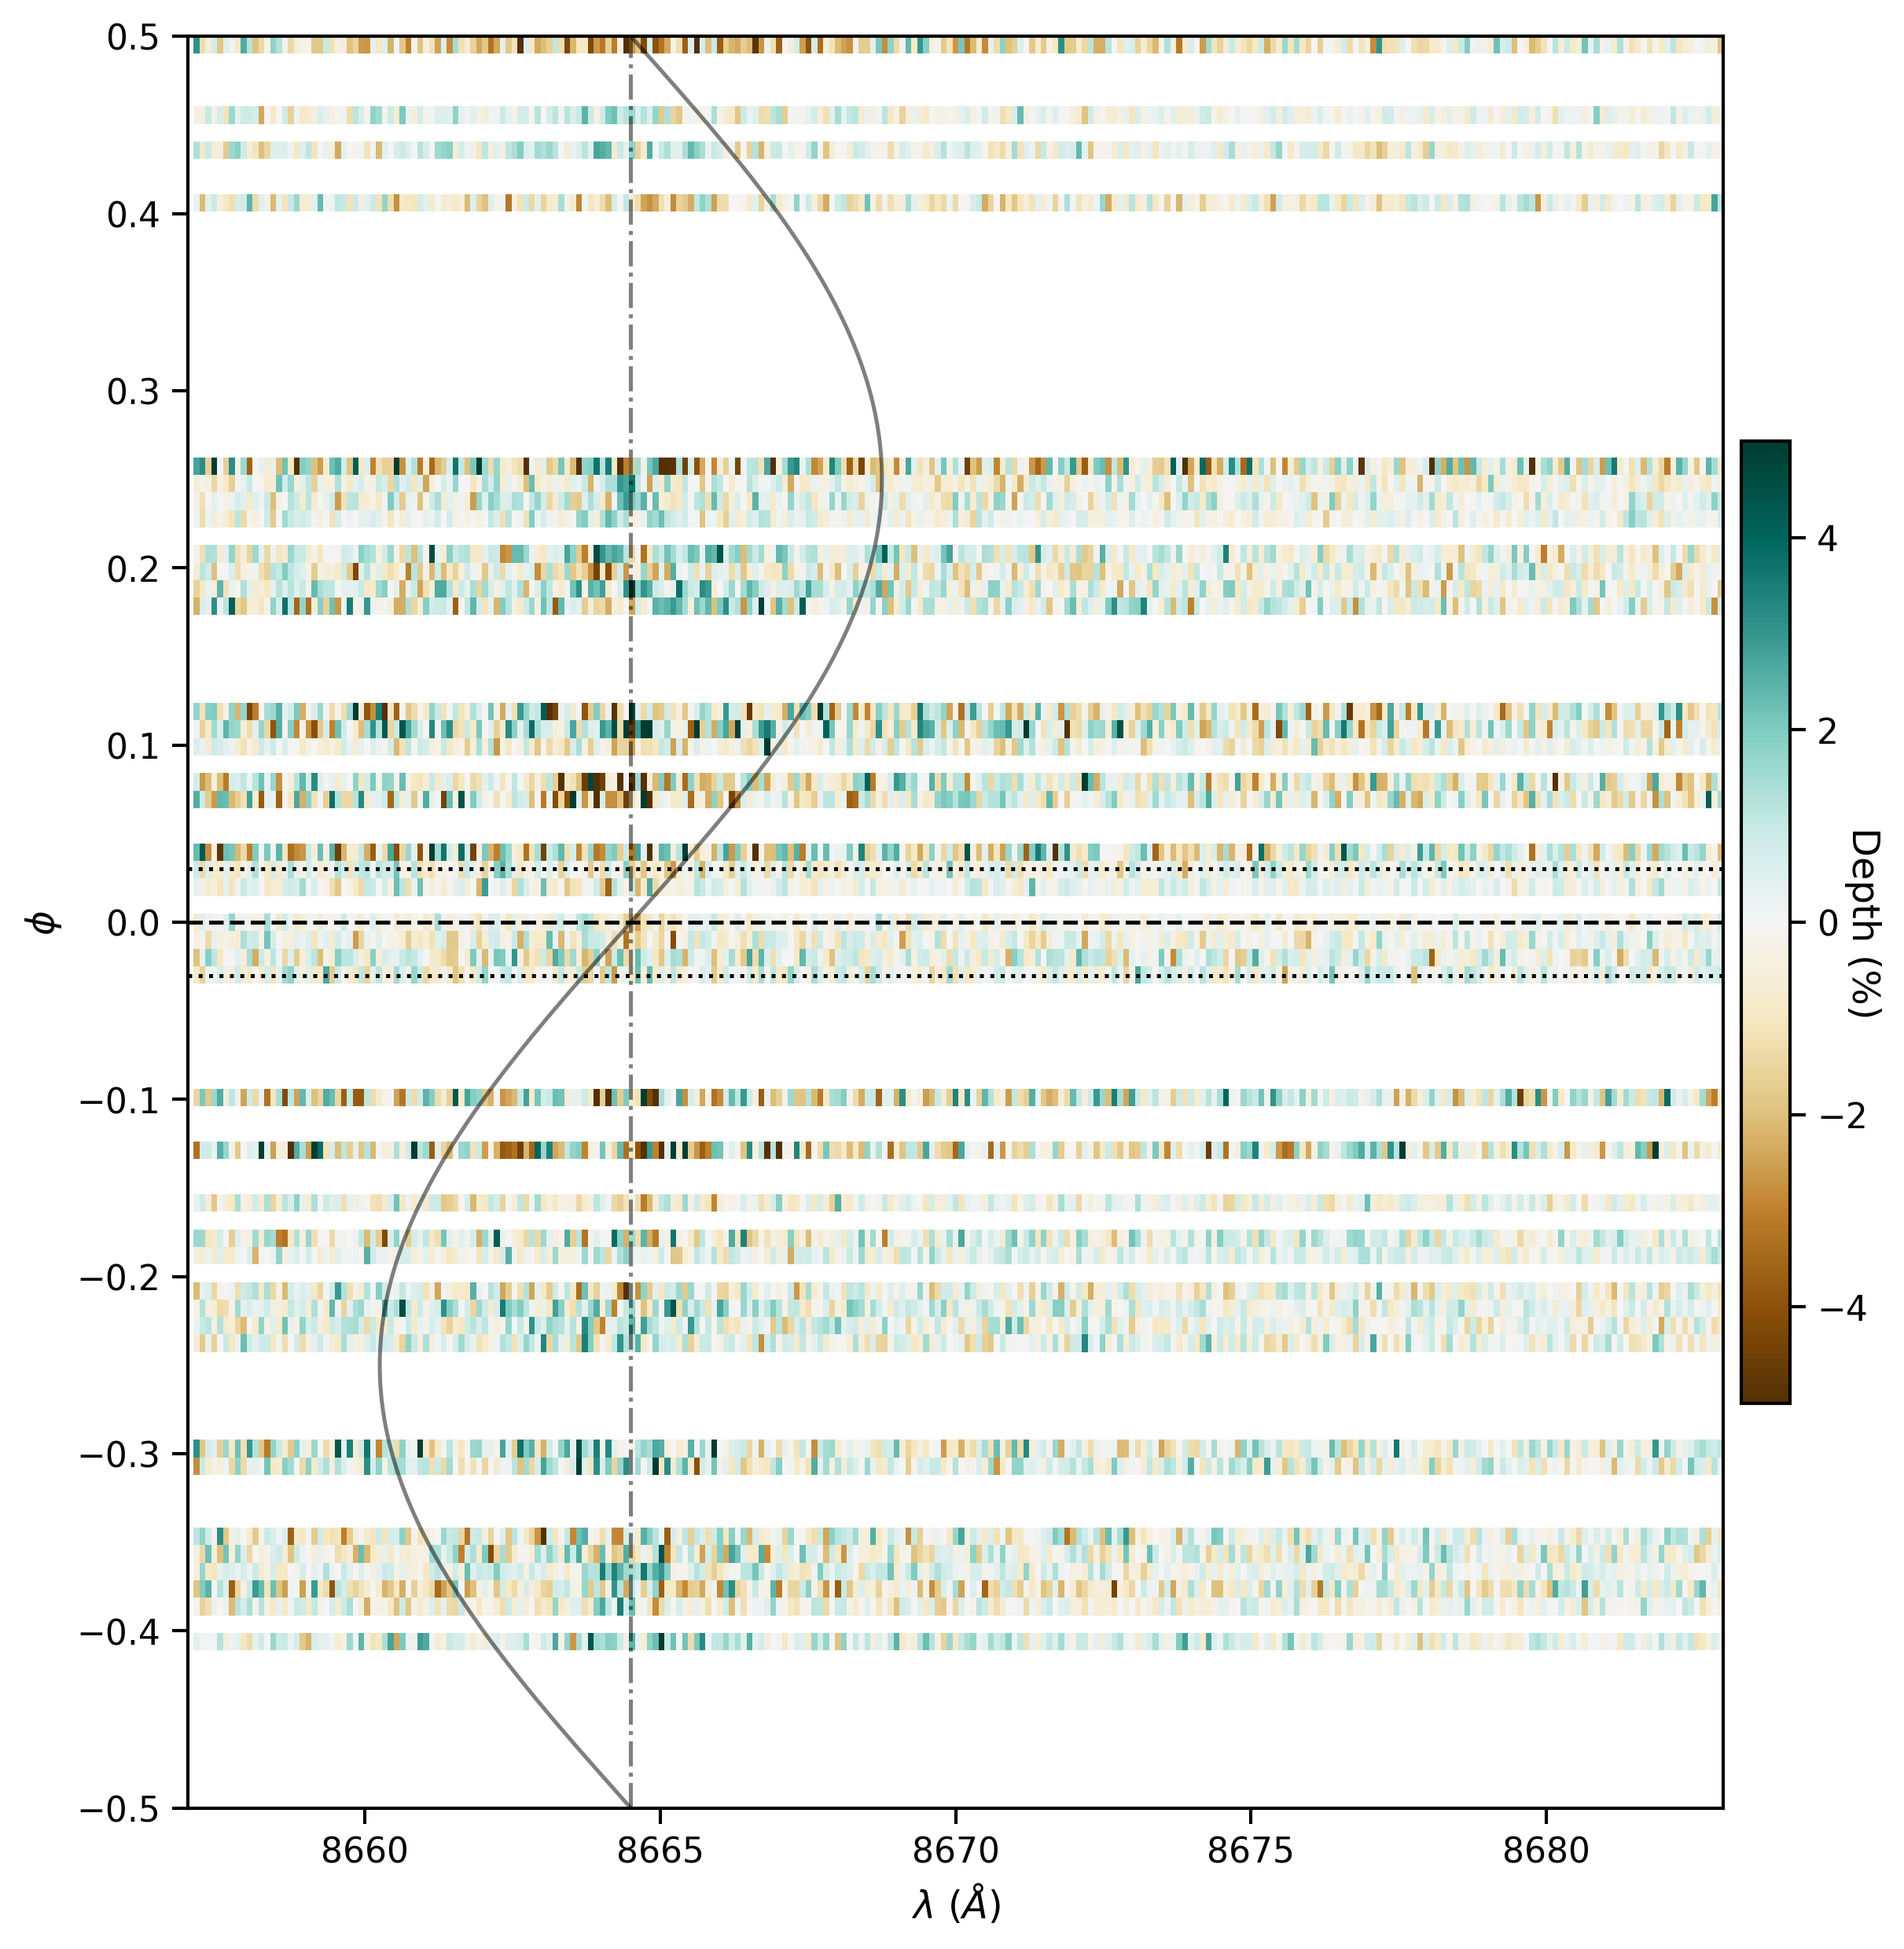
\includegraphics[width=\linewidth]{figures/Ca8662_phase_2D_diagram_resid.png}
    \caption{Non-detection of variability in the Calcium IR Triplet line at 8862 $\AA$.  No other HPF lines appear to show any variability.}
    \label{fig:CaPhaseScan}
\end{figure}

\subsection{Keck HIRES}
We retrieved 22 epochs of archival \emph{Keck HIRES} spectra via the Keck Observatory Archive (KOA). Of these, 19 were acquired through the iodine cell as reported by \citet{2017AJ....153..211Z}, providing RV orbit constraints.  The 14\arcsec~ slit height of the C2 decker appears to cause order overlap in \ion{Ca}{2} H and K lines, which contaminated the spectral extraction for 14 of the 22 spectra.  The 3\farcs5 B2 decker allowed the faithful extraction of this region for 6 spectra, which exhibit no perceptible \ion{Ca}{2} H and K variability.  The H$\alpha$ region exhibited no perceptible variability, but the timing of these spectra coincidentally missed the orbital phases ($-0.3$ to $+0.03$) where we see the greatest \ion{He}{1} 10833 \AA~ absorption excess, leaving open the possibility that detectable H$\alpha$ absorption could be present at more favorable orbital phases.  New spectra or a more careful extraction of the archival C2 decker spectra would be needed.


\subsection{Velocity substructure}
Figure \ref{fig:HeliumScanZoom} shows a zoom-in of the in-transit portion of the Helium excess absorption scan, overlaid with line center positions.  The scan appears to exhibit some velocity substructure.  At transit ingress, the absorption appears more centrally concentrated near the vertical 10833 \AA~ line.  The line depth gets slightly shallower with a slight redshift approaching transit midcenter. \authorcomment1{Add more text here and revise figure.}

\begin{figure}
    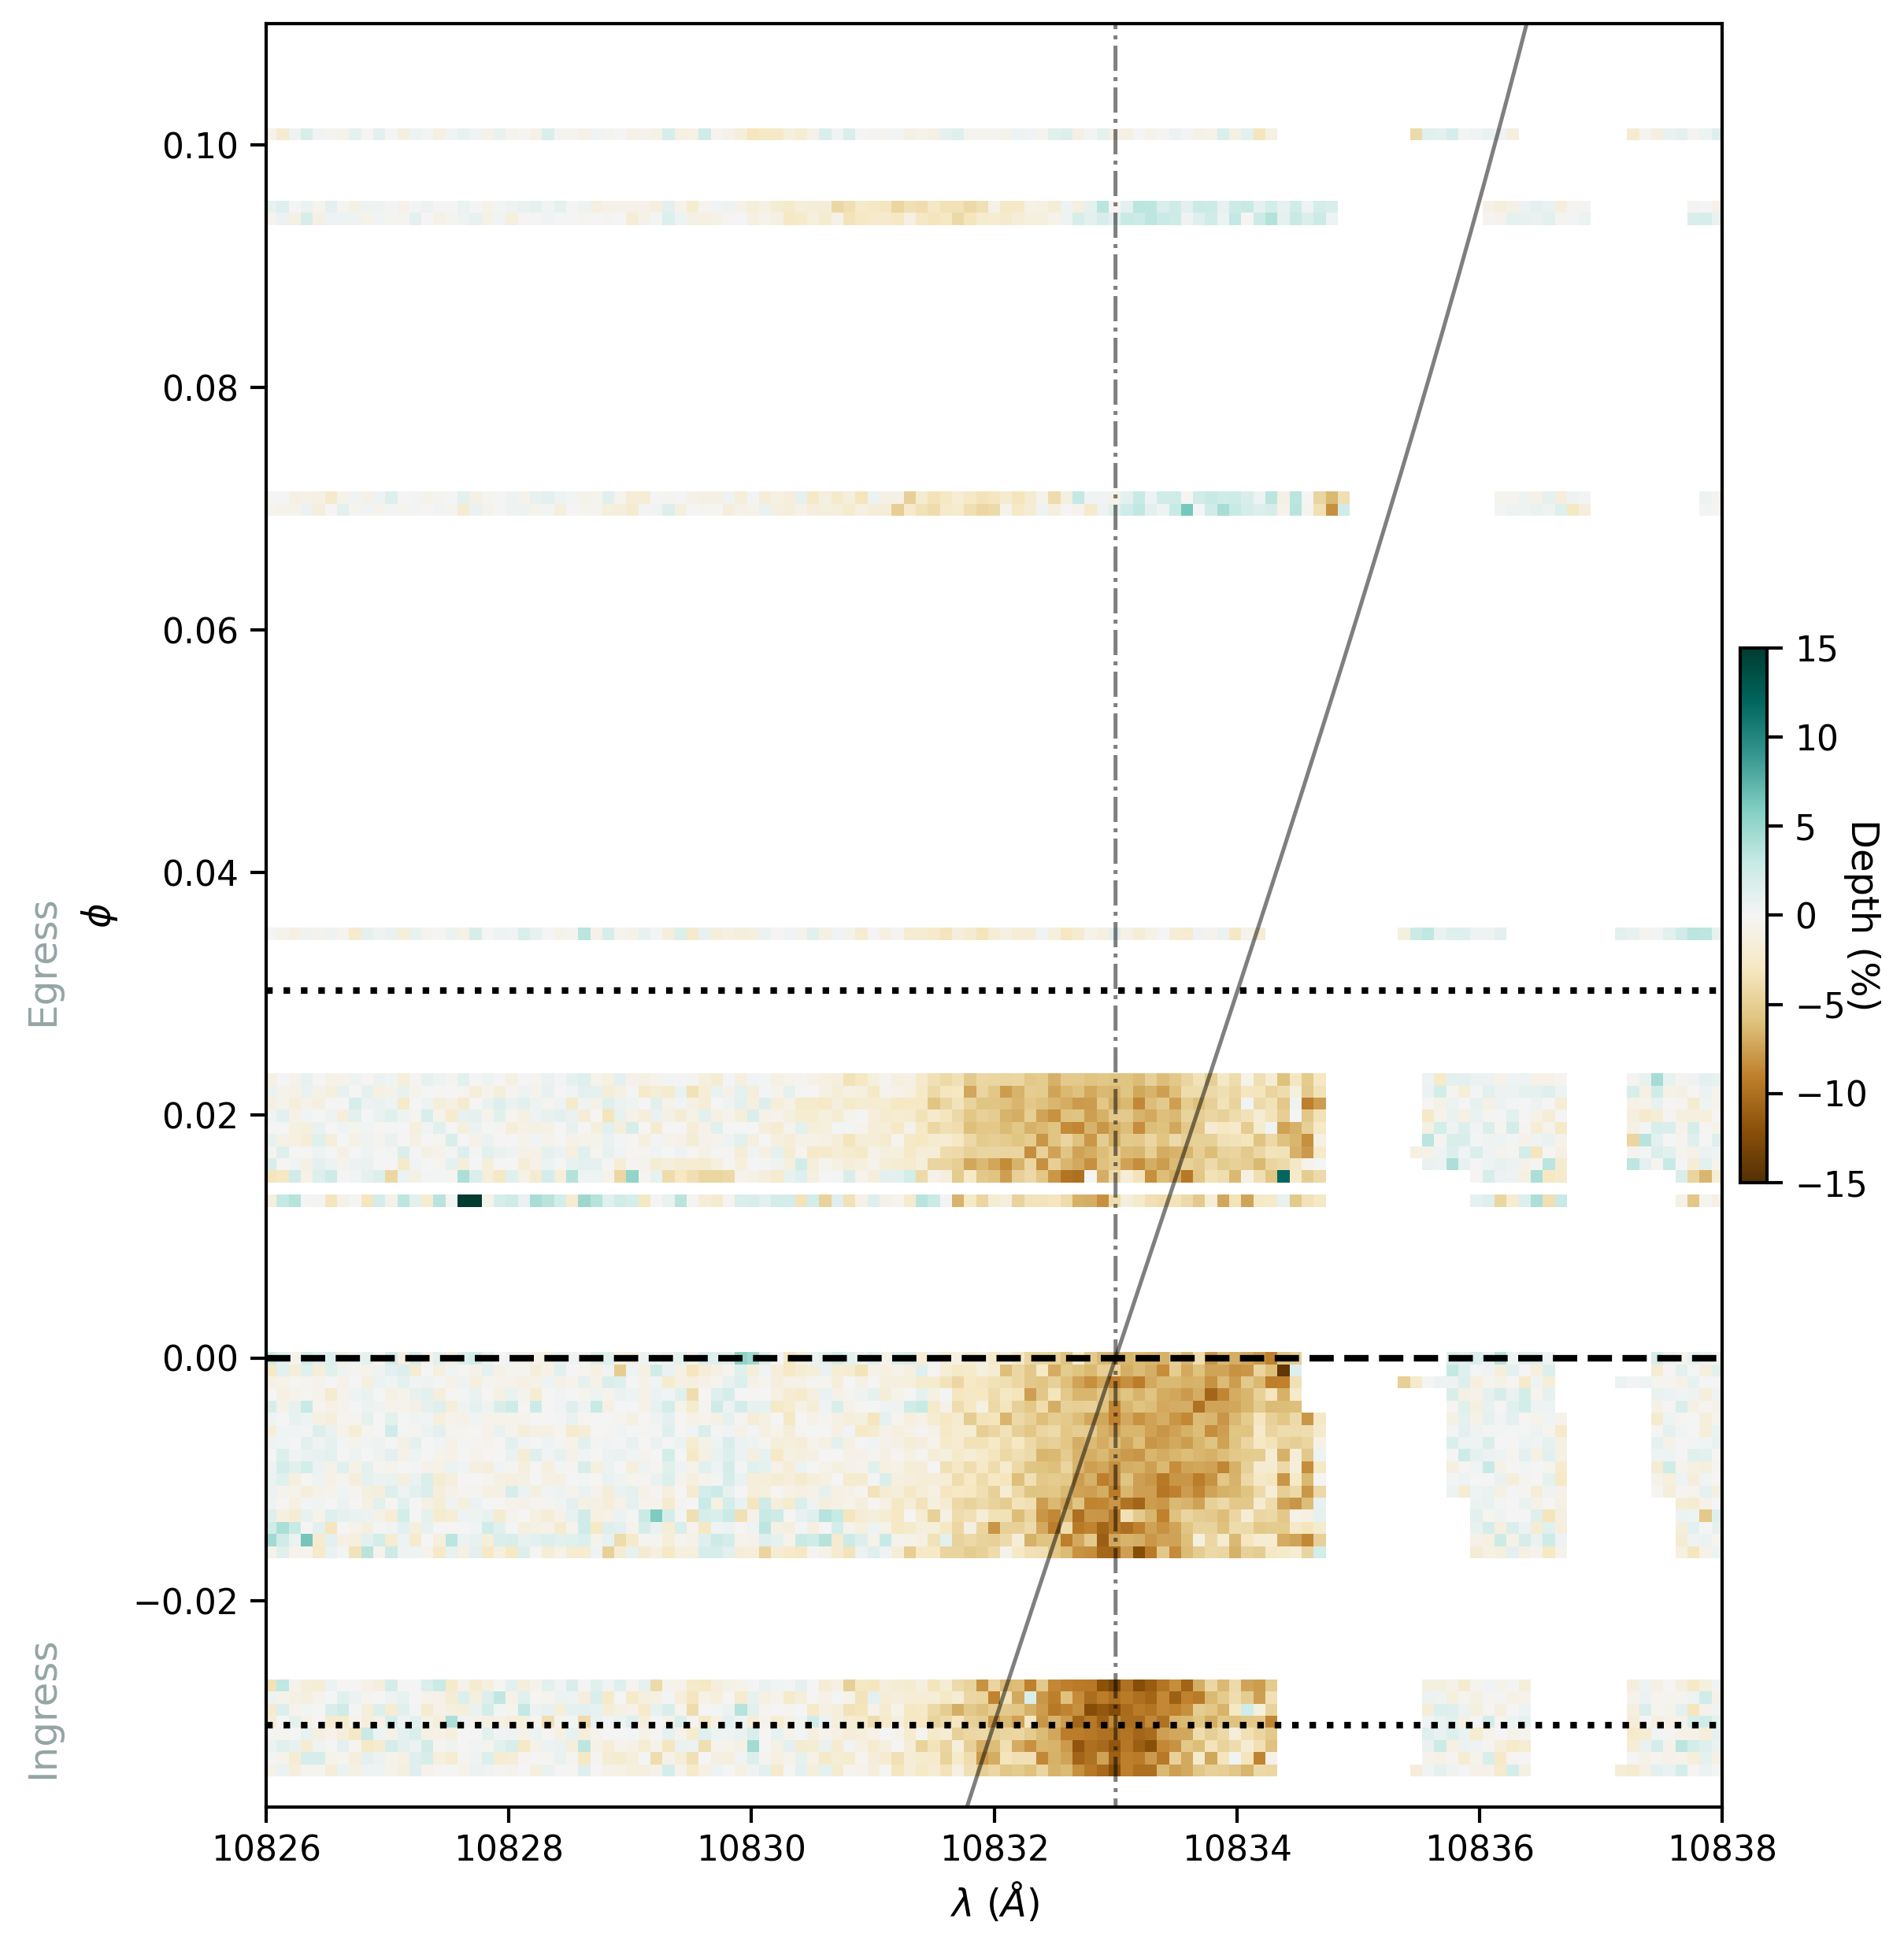
\includegraphics[width=\linewidth]{figures/phase_2D_diagram_zoom.png}
    \caption{A zoom-in of the in-transit and post-transit phase scan for the Helium 10830 triplet.  Some velocity substructure may be apparent.}
    \label{fig:HeliumScanZoom}
\end{figure}


\section{Atmospheric Escape}

\subsection{Size and geometry of outflow}
Helium absorption occurs predominantly before the planet is in-transit, indicating a \emph{leading} tail escaping the planet.  The excess occurs as early as 30\% of the orbital path.  That large fraction of an orbit translates to about 0.1 AU, 130 planetary radii, and well outside of the Roche Lobe, with its Hill radius of merely 2.6 planetary radii.  We are therefore primarily detecting gas that is entirely unbound from the planet.  The leading gas tail does not appear to accelerate, neither blue-shifting nor redshifting.   The bulk of the detectable unbound gas may therefore follow its own Keplerian trajectory at a slightly shorter period orbit, pulling away from the planet parallel to the orbital path.  Such a scenario may arise from preferential emission on the planet dayside, or other configurations that we discuss in Section \ref{secDiscuss}.

The out-of-transit excess exhibits approximately the same line width as the stellar lines, which are rotationally broadened by a $v\sin{i}$ of 30-35 km/s \citep{2017AJ....153..211Z}.  The large size of the gas stream overfills the transit chord, which means both the advancing blue side and receding red side of the rotating star are nearly continuously obscured in this spin-orbit-aligned system \citep{2017AJ....153..211Z}. The planet transits near the Stellar equator \citep{2017AJ....153..211Z}, meaning the transit chord covers about 10$\%$ of the projected stellar surface area.  Hypothetically a nearly 100$\%$ opaque optically thick stream of gas covering only the transit chord could reproduce the observed 10$\%$ absorption excess.  Alternatively---and more likely---an optically thin gas stream has some additional vertical extent perpendicular to the plane of orbit, which would act to overfill the entire projected stellar disk.  Assuming the gas has a spatially uniform optical depth of about 0.1 would reproduce the 10\% absorption excess.


\subsection{1D Parker wind models and mass loss rates}\label{pwinds}
The dramatic leading tail of atmospheric escape suggests that more complicated 3D hydrodymaic simulations coupled with stellar wind \citep{2022ApJ...926..226M} may be needed to depict the geometry faithfully.  Here we explore one-dimensional (1D) models, which offer ease of interpretation and rapid calculation.  We employ the open-source \texttt{p-winds} code \citep{2022A&A...659A..62D}, which implements a transonic 1D Parker wind model with radiative transfer of the Helium 10830 triplet \citep{2018ApJ...855L..11O,2020A&A...636A..13L}.

The predicted Helium ionization depends sensitively on the XUV flux \citep{2019ApJ...881..133O}.  Ideally we would have a measurement of the XUV spectrum of \hatp, but the limited facilities and distance of the source preclude these challenging observations.  Instead we constructed panchromatic X-ray to visible SEDs by scaling and stitching together synthetic spectra to provide a range of high and low $L_X/L_\mathrm{bol}$.  We chose a 6400 K PHOENIX \citep{husser13} solar metallicity photospheric spectral template with $\log{g}=3.5$, scaled to the solid angle seen by \hatpb.  The F7IV-V \object[tau Boo]{$\tau$ Boo} serves as the closest analog with synthetic x-ray coronal spectra available \citep{2011A&A...532A...6S}.  But \hatp resides closer to the Kraft break than does \object[tau Boo]{$\tau$ Boo}, and the move to hotter F stars may be associated with rapid changes in the stellar wind and other atmospheric changes leading to the prospect of much lower XUV luminosity for \hatp.  So there remains significant uncertainty about the applicability of the \object[tau Boo]{$\tau$ Boo} x-ray spectrum to \hatp.  We scaled the synthetic SED of \object[tau Boo]{$\tau$ Boo} retrieved from X-exoplanets \citep{2011A&A...532A...6S} so that the integral of ground-state ionizing photons ($\lambda<504\AA$) exhibited $L_X/L_\mathrm{bol} \in [10^{-7}, 10^{-5}]$.  Figure \ref{fig:XUV} shows two conceivable SEDs with a high and low radiation hardness.

\begin{figure}
    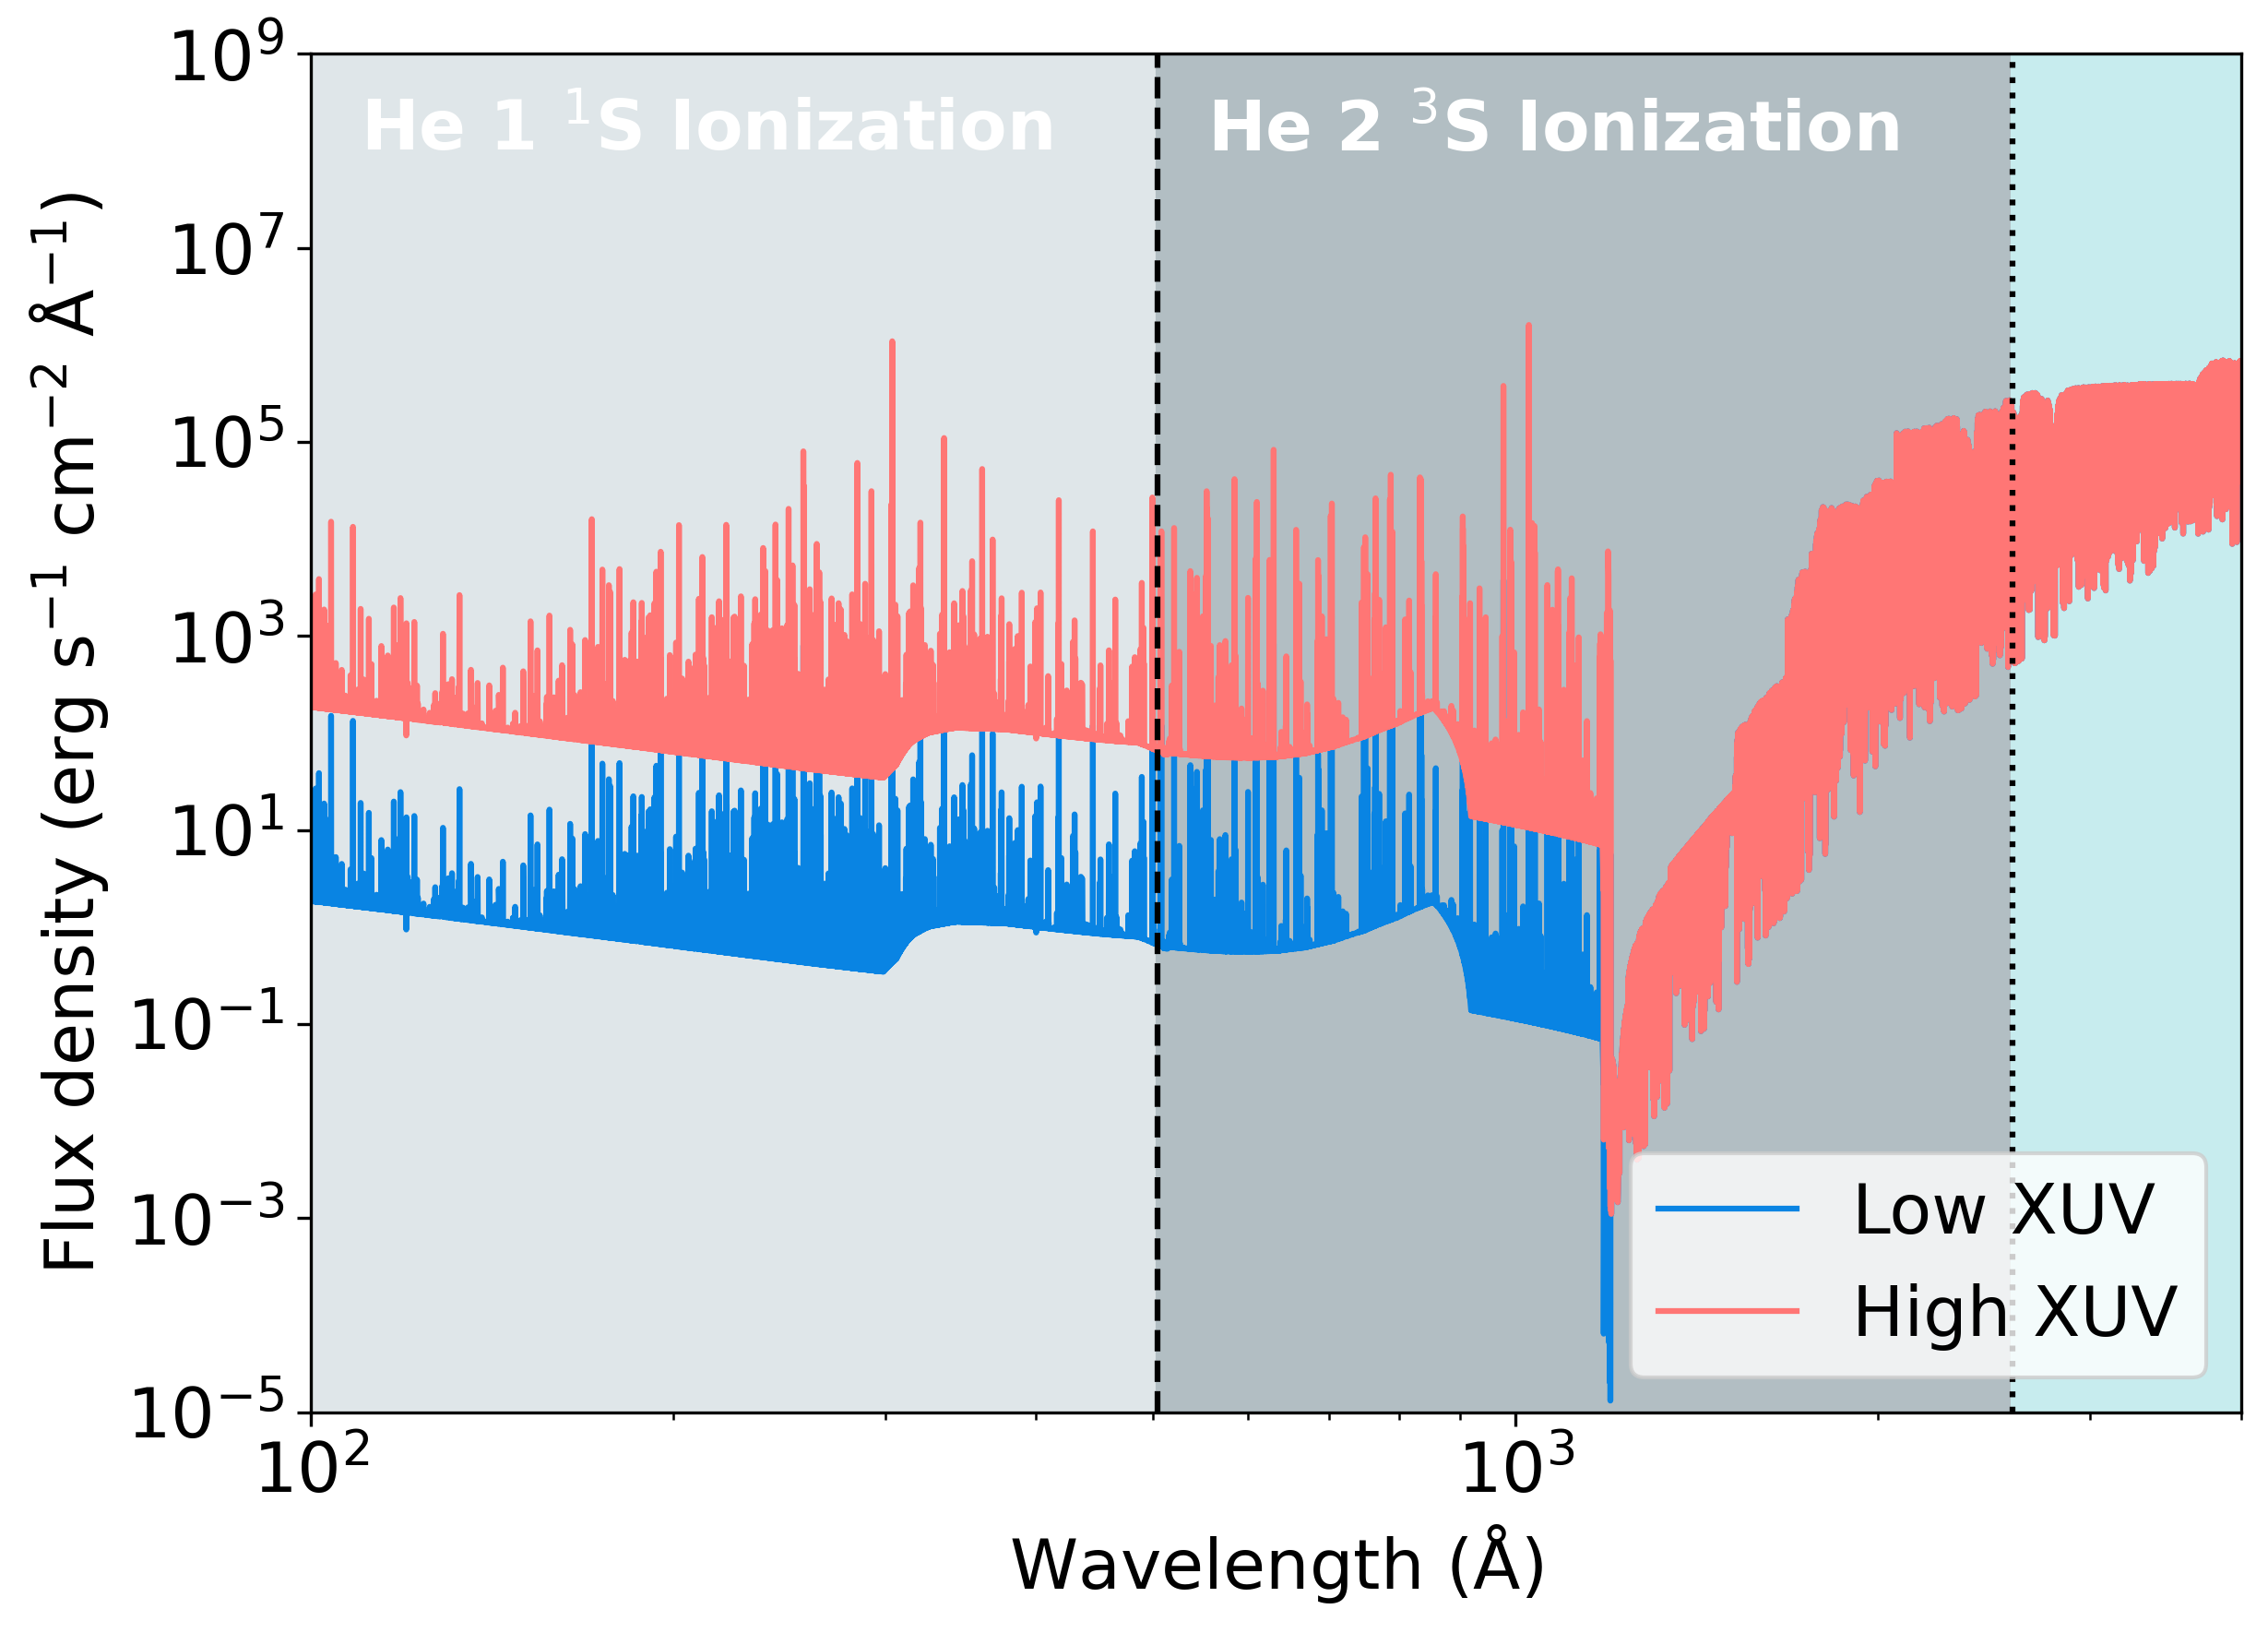
\includegraphics[width=\linewidth]{figures/XUV_flux_schematic.png}
    \caption{Synthetic XUV radiation scenarios for \hatpb.  }
    \label{fig:XUV}
\end{figure}

The SED shows two key features.   First the corona model does not extend all the way to 2600 $\AA$ photons capable of ionizing out of the 2 $^3$S Helium metastable state.  This apparent deficit probably does not matter because the F spectral type obtains most of its NUV photons ($\lambda\sim2600\AA$) from the Wein side of the photospheric spectrum, so the hardness of the radiation stems mostly from the assumptions of the corona flux level.  The wavelength-dependent cross section for absorption (not shown) is largest just blueward of the ionization thresholds, so the differences in the spectrum between 504 $\AA$ and 1000 $\AA$ have relatively little impact on the overall ionization out of the metastable state.

Equipped with these three SEDs of differing radiation hardness, we explored different mass loss rates and exosphere temperatures.  Figure \ref{fig:pwinds} shows one example model spectrum with $\dot{M} = 7\times10^{13}$ g/s, and $T_0=9100$~K, with the high XUV spectrum ($L_x/L_\mathrm{bol}=10^{-4}$).  The model spectrum exhibits approximately the same line width and depth as our HPF observations, making it a conceivable solution.

At least a few shortcomings limit the applicability of this 1D Parker wind model.  First, the model-dependent line profile (\emph{i.e. width and depth}) is degenerate with XUV flux, $\dot{M}$, and $T_0$, and so a range of these parameters can be fine-tuned to obtain a large range of mass loss rates consistent with the data and our limited understanding of the XUV flux.  Second, the 1D model breaks down when attempting to explain the inherently 3D leading tail geometry.  We discuss these two and other model-dependent interpretations in Section \ref{secDiscuss}.




\begin{figure}
    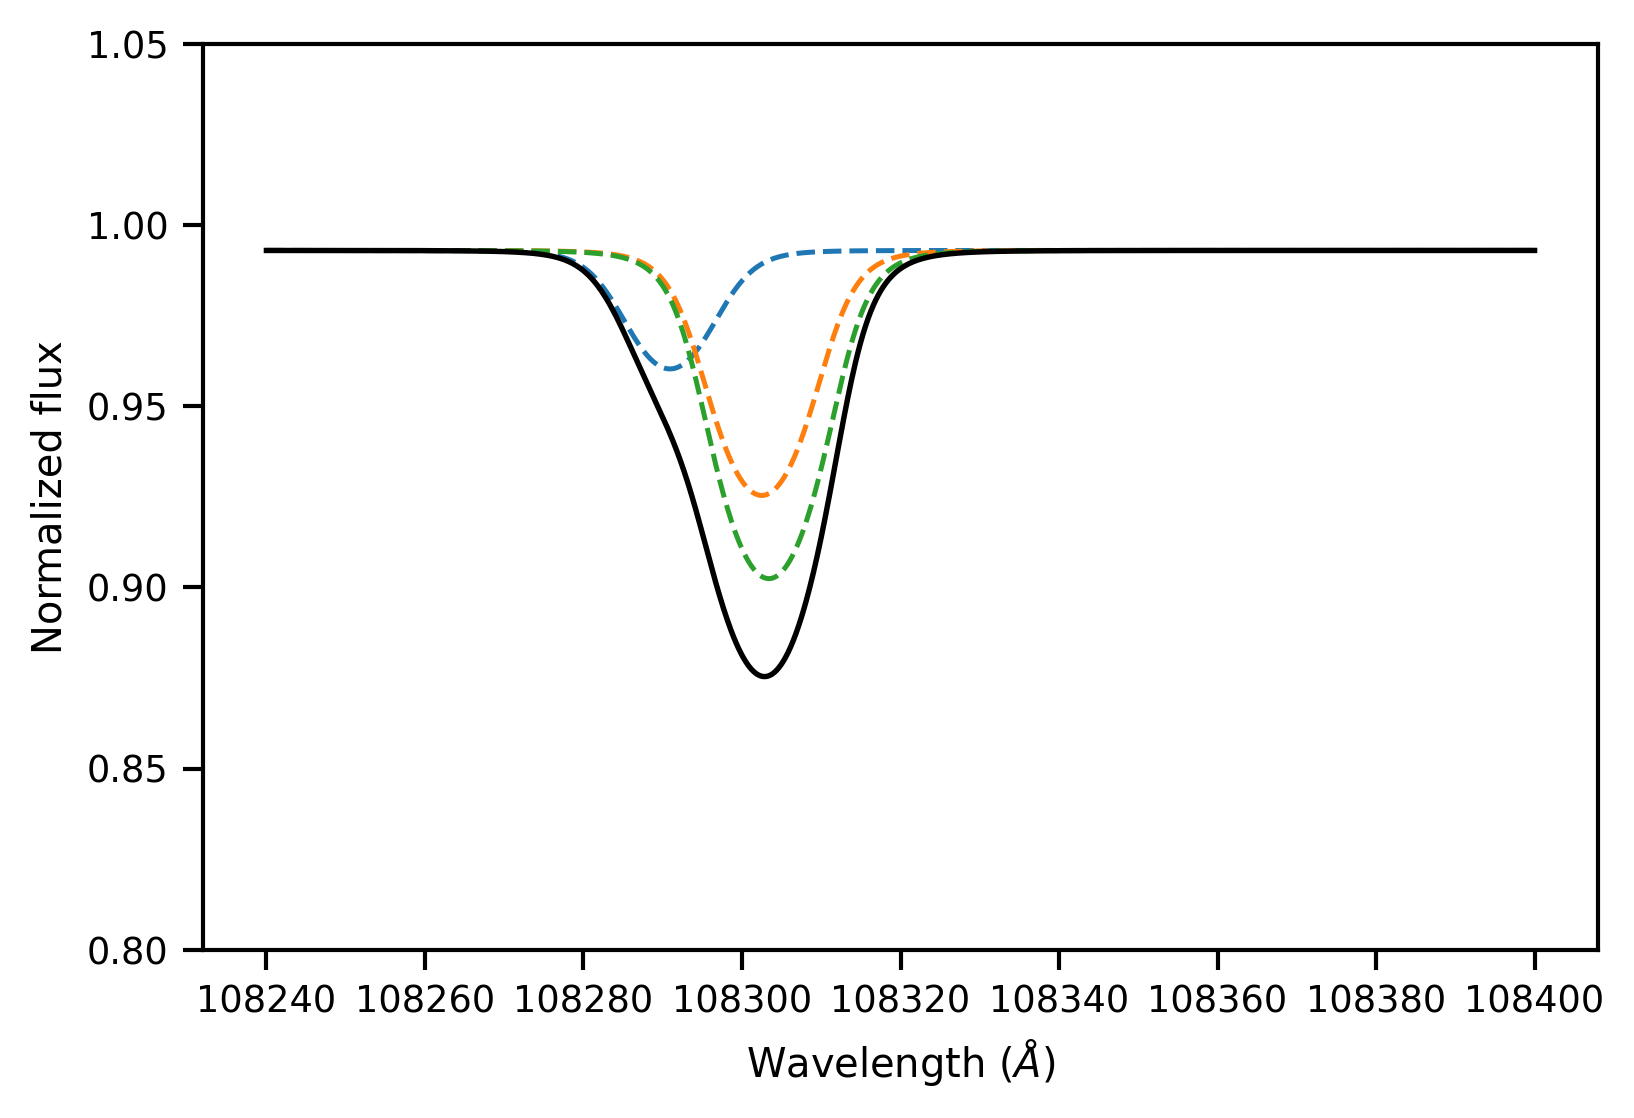
\includegraphics[width=\linewidth]{figures/pwinds_1D_higXUV_t1p2Gyr.png}
    \caption{Simulated 1D Parker wind model of Helium absorption in \hatpb.  The spectrum was generated with a mass loss rate of $1.7\times10^{13}$ g/s, exosphere gas temperature of 9100 K, and with the high XUV spectrum ($L_x/L_\mathrm{bol}=10^{-4}$) shown in Figure \ref{fig:XUV}.  The line depth and width broadly agrees with the width observed in HPF.}
    \label{fig:pwinds}
\end{figure}



\section{Discussion} \label{secDiscuss}

\subsection{Ohmic Dissipation and runaway escape}
\object{HAT-P-67 b} exhibits both dramatic atmospheric escape and significant radius inflation.  Ohmic dissipation stands out as a physical mechanism that could be responsible for both of these attributes.  \citet{2011ApJ...738....1B} showed that ohmic heating acts to inflate hot Jupiters, with low mass hot Jupiters overflowing their Roche lobes and leading to evaporation on Gyr timescales.  The Ohmic heating scenario requires only on a modest planetary magnetic field ($\sim$1 G) and enough photoionization to ionize some modest fraction of neutral metals.  The ``sweet spot'' for this phenomenon appears to prefer equilibrium temperatures in the range of $1500<T_\mathrm{eq}<2000$ K \citep{2011ApJ...738....1B}, well matched to HAT-P-67 b's $\sim$1900 K.  A plausible scaling law relationship approximate to an order-of-magnitude predicts an inflation timescales (Eq. 20 in \citet{2011ApJ...738....1B}):
\begin{equation}
    \tau_{\textit{infl}}\sim \left(\frac{0.01}{\epsilon} \right) \left(\frac{M}{M_{J}}\right)^2 \left(\frac{R_{J}}{R}\right)^3 \left(\frac{1500 \textrm{K}}{T_\mathrm{eff}}\right)^4 \textrm{Gyr}. \label{eqInflate}
\end{equation}


\noindent yielding an incredibly short 5 Myr timescale for \hatpb, assuming a typical $\epsilon\sim0.01$. The order of magnitude of this inflation timescale is so fleetingly short that \hatpb must be in the runaway stage of inflation, rapidly losing mass, and growing in surface area to fuel a positive feedback loop.

\subsection{Photoevaporation}
The prospect of Ohmic dissipation does not preclude the possibility that other mass loss drivers are at play.  Photoevaporation should simultaneously drive heating of the upper layers in the atmosphere, reinforcing the mass loss associated with Ohmic dissipation.  It is not clear which effect predominates.


\subsection{Constraining mass loss rate}
A 5 Myr inflation timescale would imply an instantaneous $\dot{M}_\mathrm{infl}\sim10^{15}$ g/s, about 50 times larger than the 1D Parker wind model mass loss rate of $\dot{M}_\mathrm{1D}\sim2\times10^{13}$. Here we enumerate all of uncertainties that go into assessing mass loss rates to show that some in-between mass loss rate may be plausible.

First, the scaling law arguments that produced Equation \ref{eqInflate} (Eq. 20 of \citet{2011ApJ...738....1B}) were only proposed as order of magnitude estimates not to be taken too faithfully.  So a $10\times$ higher inflation timescale of 50 Myr would yield $\dot{M}_\mathrm{infl}\sim10^{14}$ g/s, still a very large mass loss rate, but only a factor of 5 away from the baseline 1D model.  Order unity uncertainties in the Ohmic dissipation efficiency $\epsilon$ may also contribute.

As mentioned in Section \ref{pwinds}, inferring the mass loss rate from observations is strongly model dependent, as seen in \censorbox{cite e.g. S.V. papers}.  The XUV flux, exosphere temperature $T_0$, and $\dot{M}$ are all at least partially degenerate.  In particular, the uncertain XUV-to-NUV flux ratio confounds the interpretation of the observed Helium signal.  Even the ``high XUV'' scenario in Figure \ref{fig:XUV} does not have enough ground-state ionizing photons to penetrate to within 5 $R_p$ of the planet surface.  This means that at best only 1 in $10^{6}$ Helium atoms participate in the observability of the Helium metastable triplet lines in the baseline 1D Parker wind model.  Turning down the XUV flux makes the signal even less observable.  A larger mass loss rate would be needed to explain the same observed HPF Helium absorption, if say only 1 in $10^{7}$ helium atoms are populating the metastable state.

Finally, the entire premise of the Parker wind model may be unjustified due to the inherently 3D geometry of the leading tail.  In the next section we critically examine the assumptions in the 1D Parker wind model.

\subsection{Causes for the leading tail}
Several physical phenomena could give rise to a leading tail geometry.  Here we explore two leading candidates: orbital shear and stellar wind confinement.

Figure \ref{fig:KeplerianShear} shows an illustration of Keplerian shear adapted to the system properties of \hatpb.  In this scenario, the wind launches primarily from the dayside, with relatively little or no wind launched from the nightside.  The wind initially launches radially from the planet, with the strongest wind located near the sub-stellar point, the line connecting the planet to star along the vertical axis in the figure.  Inefficient heating near the terminator subdues the mass loss in the $x-$direction, meaning that this wind exhibits not a hemi-spherical shape, more like a bulb or torpedo.  The gas increasingly experiences the star's Keplerian potential past the Roche lobe, accelerating in the direction of orbital motion, $+x$.  The accelerating column eventually overtakes the planet completely, with the prospect of extending to hundreds of planetary radii.

\begin{figure}
    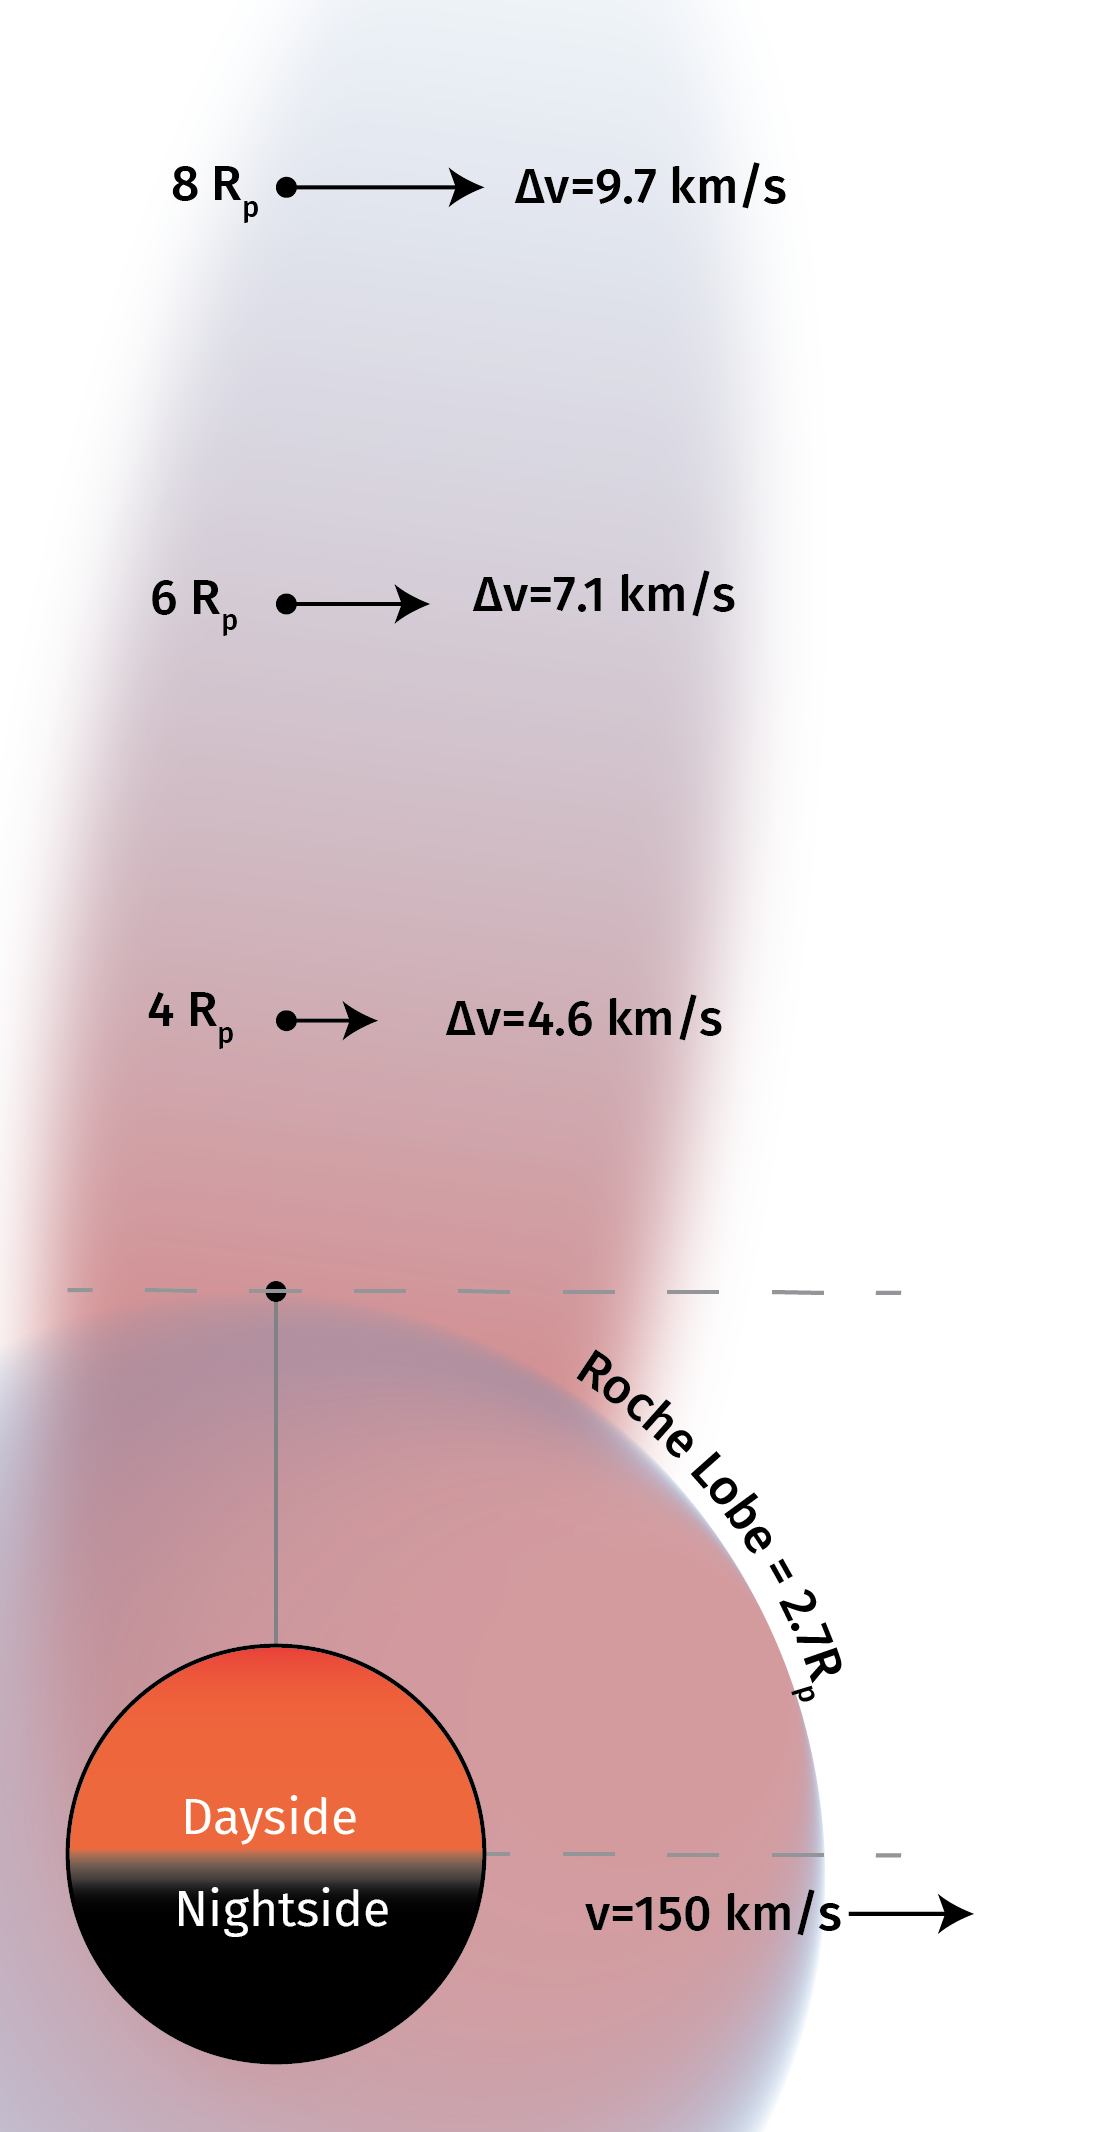
\includegraphics[width=0.8\linewidth]{figures/KeplerianShear_v0p3.png}
    \caption{Schematic of Keplerian orbital shear.  Locations outside the Roche lobe experience orbital shear from the Keplerian potential.  A wind launched primarily from the dayside will tend to form a leading tail.}
    \label{fig:KeplerianShear}
\end{figure}


Stellar wind confinement arises from a bow-shock configuration, in which the planetary wind encounters the stellar wind and a shock front causes a density enhancement.  A trailing tail may be present, but would not undergo the same boost in density, and would be rapidly carried away by the stellar wind.  This asymmetry could yield the appearance of a leading tail even if mass loss proceeds isotropically, or the asymmetry could be reinforced by an additional dayside/nightside asymmetry.  Examples of this asymmetry can be seen in 3D MHD modeling of WASP 107~b \citep{2022ApJ...926..226M}.


%\begin{figure*}[t]
%    \includegraphics[width=\linewidth]{figures/murray_clay_schematic_v0p2.png}
%    \caption{Schematic of the relevant length scales in a stratified atmosphere, modeled after Figure 8 from \citet{2009ApJ...693...23M}.  The sonic point resides at a mere 2 atmospheric scale heights, and well below the photoionization level of Hydrogen, raising the possibility that the supersonic flow begins neutral and becomes ionized later on.}
%    \label{fig:murrayClaySchematic}
%\end{figure*}

\subsection{The Ohmic Dissipation Cliff: Evaporative annihilation as the cause of a lack of sub-Saturns}
The Ohmic dissipation mechanism predicts a rapid inflation timescale leading to the complete evaporation of hot Saturns.  The Ohmic dissipation mechanism made two key observable predictions.  The Ohmic dissipation heating should become less efficient as irradiation increased past an equilibrium temperature of about 2000 K.  Second, hot Saturns should should runaway evaporation, whereas hot Jupiters should reach equilibrium---albeit inflated---radii after Gyr timescales.  Both of these outcomes predated data that could adequately validate them, and these outcomes differ from the behavior of other heating mechanisms, such as photoevaporation or tides.

\citet{2018AJ....155..214T} statistically favored Ohmic dissipation based on evidence for a turnover in the heating efficiency of hot Jupiters in a sample of 281 Giant planets.  Futhermore, \citet{2018AJ....155..214T} also highlighted the lack of inflated sub-Saturns as an anomaly: the observational capability exist to detect such sources in large numbers and yet they were not found.

\begin{figure}
    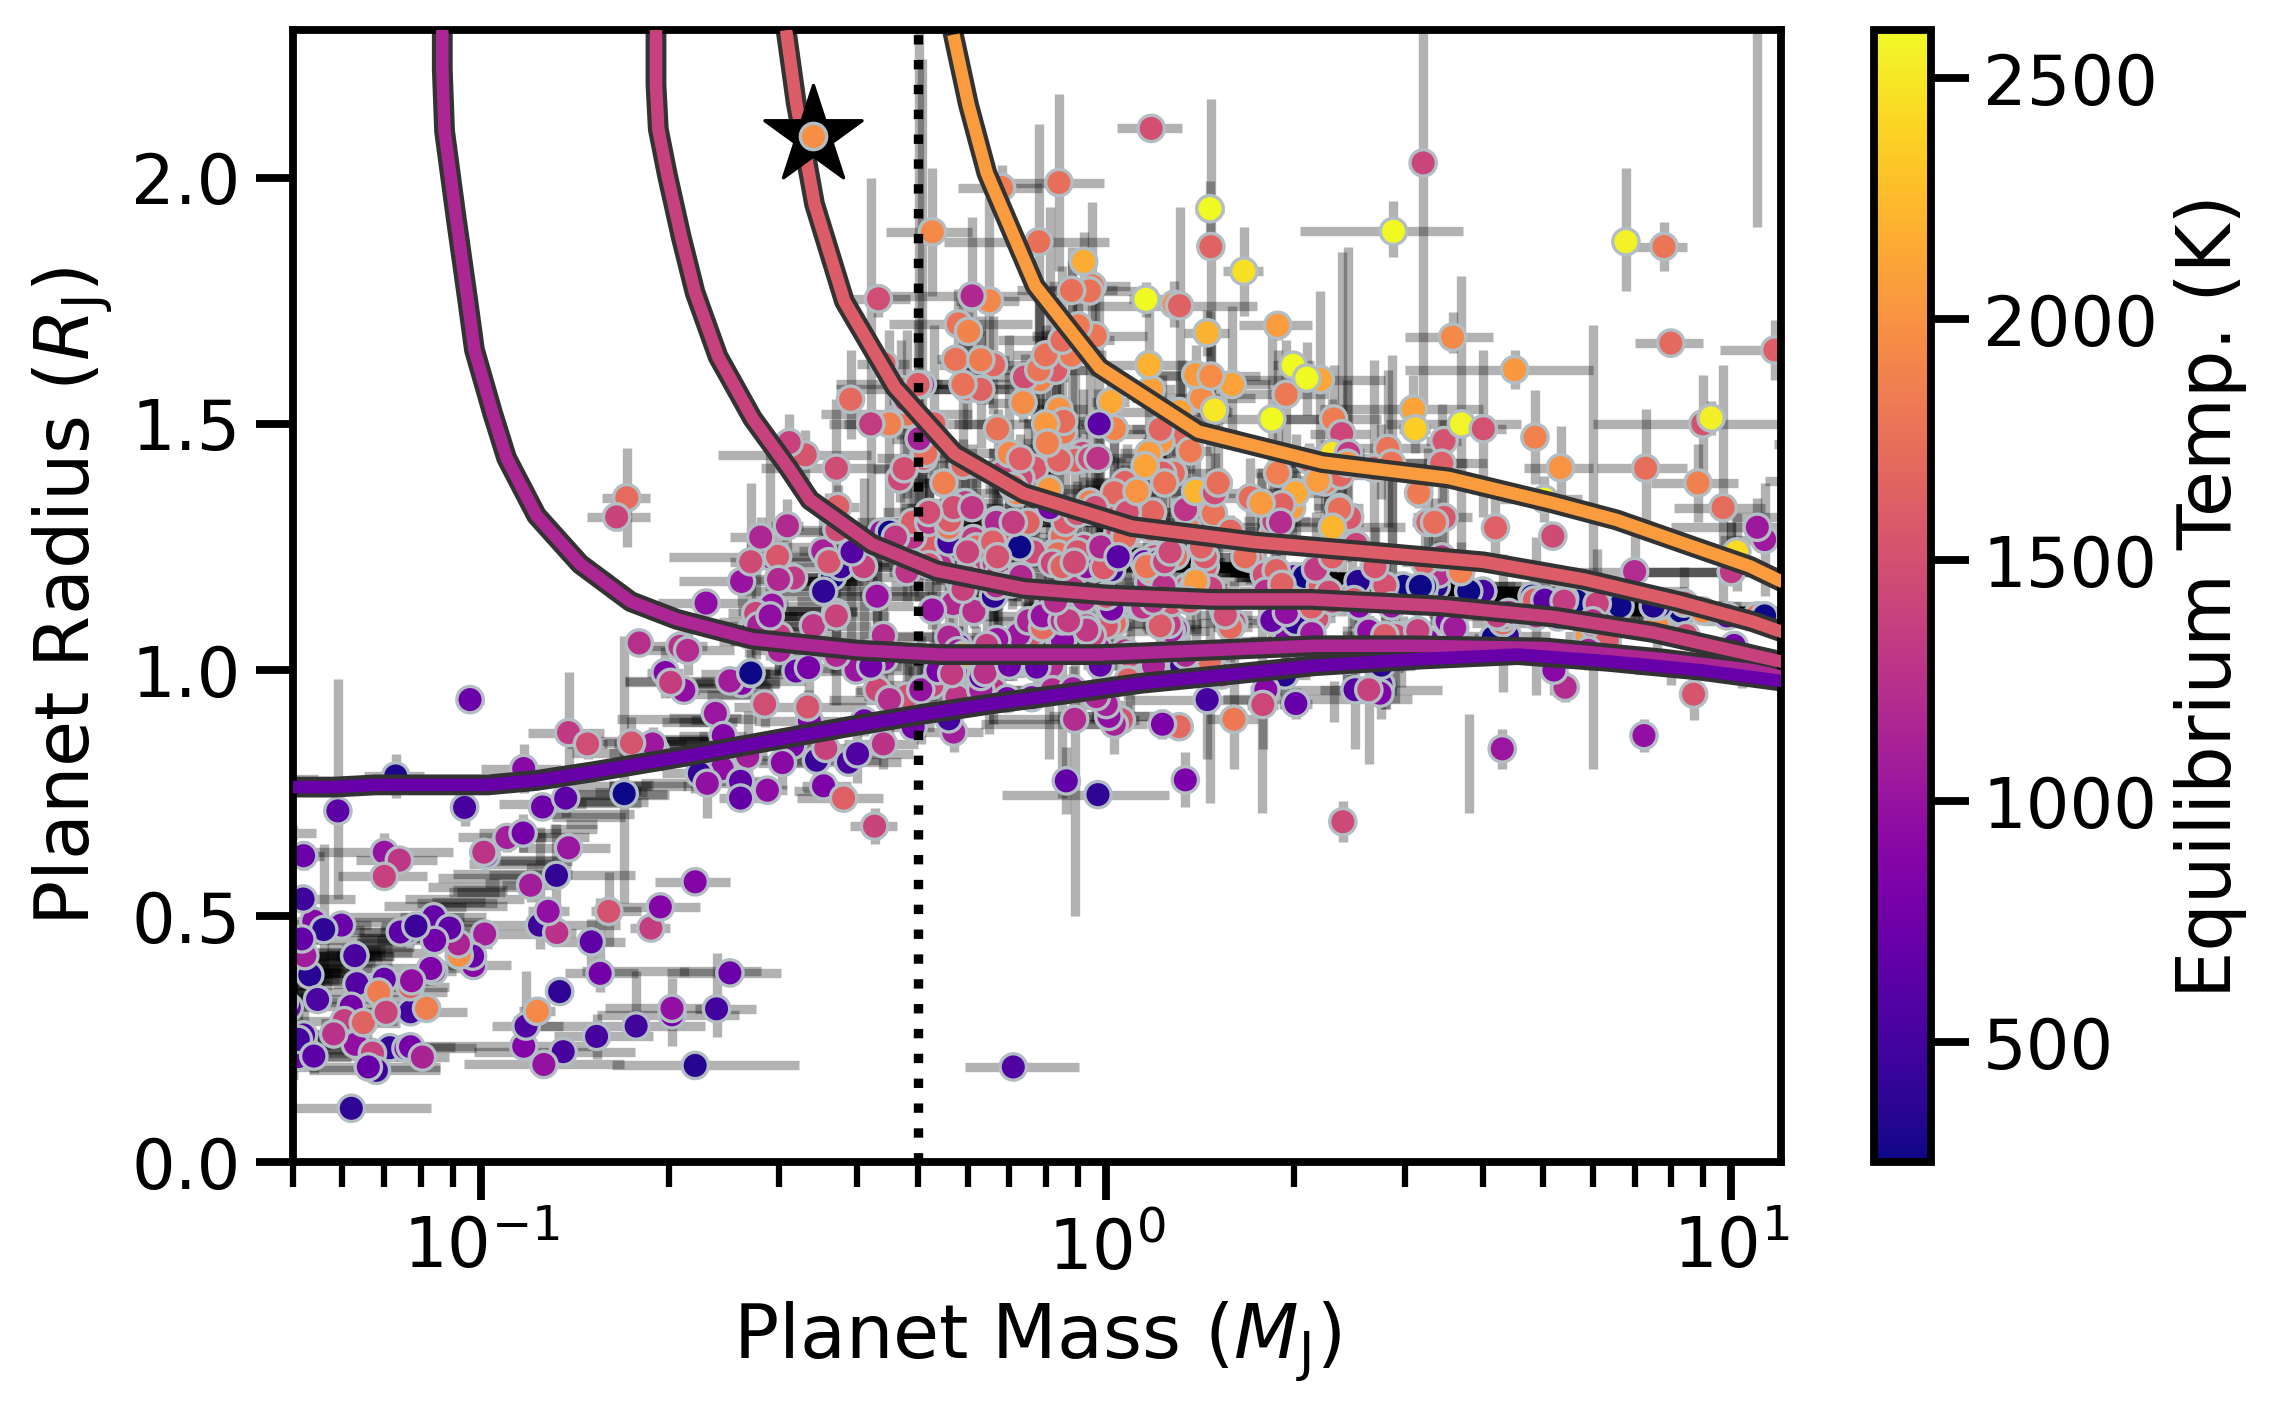
\includegraphics[width=\linewidth]{figures/tf2018_fig2_update2023_HAT.png}
    \caption{Mass-radius trends for inflated hot sub-Saturns and hot Jupiters, form modeled after Figure 2 from \citet{2018AJ....155..214T} and updated with NASA Exoplanet Archive confirmed planets.  The trend lines show mass-radius relationship for equilibrium temperatures of 500, 1000, 1250, 1500, and 2000 K, assuming the mean composition and mean heating efficiency from the original figure.  HAT-P-67~b stands alones as occupying the ``Ohmic Dissipation Ridge'', defined by the lack of inflated sub-Saturns, and explained by short lifetimes form runaway inflation and mass loss.}
    \label{fig:murrayClaySchematic}
\end{figure}

This dearth of hot-Saturns has persisted into the \emph{TESS} era.  Figure XX highlights the region of highly irradiated close-in planets with $N=$\censor{x} planets accessed through the NASA Exoplanet Archive \censor{cite NExScI}.  \hatpb occupies a relative void in this region.

The observation that \hatpb---the only hot Saturn searched for atmospheric escape to date---exhibits mass loss indicative of a terminal fate leads us to a natural explanation for the dearth of inflated hot Saturns.  The inflationary lifetime of this class is so short that observing planets of this class is unlikely.  \hatpb appears to be one of the rare planets that we happen to catch a glimpse of before it has been completely annihilated.

We therefore attribute this cliff in the $m_p$ vs $R_p$ diagram to Ohmic dissipation.  \citet{2018AJ....155..214T} emphasized the positive feedback loop as a cause for the lack of sub-Saturns, and noted an alternative interpretation-- mass-dependent migration segregation.  While both scenarios are conceivable, the evidence of strong evaporation of \hatpb favors the evaporation scenario.  Futhermore, the runaway evaporation of hot-Saturns was naturally predicted by the Ohmic dissipation mechanism, whereas mass-dependent migration has only been developed as a post-diction.


We predict that the few other inflated hot-Saturn \hatpb-analogs should also show evidence for atmospheric escape.  These sources make excellent targets for \ion{He}{1} 10830 observations, and other atmospheric escape diagnostics.  The key figure-of-merit can be distilled to $\tau_\mathrm{infl}$, and ignoring the $\epsilon$ term.  Following \censor{Kempton} et al we define a Helium Spectroscopy Metric (HSM) defined as...


\subsection{Cause for stellar modulation}
The \emph{TESS} lightcurve exhibits up to $0.36\%$ peak-to-valley modulation amplitude, with a characteristic timescale of $p=4.8-5.2$ days. Some sectors exhibit lower amplitudes.  The conventional interpretation would consign these cyclical modulations to the familiar stellar activity: surface features---either starspots, faculae, or plage---entering and exiting the projected stellar disk on the stellar rotation period comparable to the 4.8 day orbital period of planet b.  The cause for such orbital and rotational synchronization would then ostensibly be tides.  We examine the prospect of tides in the next subsection.

Alternatively, the exteme mass loss and credibility of the ohmic diffusion model motivates the prospect of Star Planet Magnetic Interaction (SPMI) that we consider now.  In this scenario, the magnetic field of the planet permeates the space between the star and planet.  Magnetic perturbations propagate via planetary magnetic fields with the Alfv\'en speed.  The planet can interact with the star if the Alfv\'en speed exceeds the stellar wind speed controling the bulk motion of intervening medium.  The magnetic field of the planet is not known, but the ohmic dissipation mechanism favors a limited range in the magnetic field strength: large enough to cause significant dissipative energy generation, but not too large to shut down charged particle motion entirely.  \citet{2011ApJ...738....1B} estimate this range as between about 1-30~G.

The non-detection of variability in the \ion{Ca}{2} H and K lines and H~$\alpha$ lines appears to disfavor this SPMI interpretation.

%\subsection{Timescale for tidal synchronization}


%\subsection{Hot Spot Scenario}
%The TESS 0.2\% flux variation could hypothetically arise from the foot-print of a star-planet interaction. Assuming that this increase in flux is due to a hot spot with a contrast of 200\% the ambient photosphere in the TESS bandpass, the hot spot would have a modest 5\% coverage fraction.  Thermal radiation from gravitational infall alone cannot explain the luminosity of this spot, so it would have to stem from a non-thermal cause.

%\subsection{Tidal Locking Calculation}
%The similarity of the rotation period with the orbital period suggests the star-planet system may be tidally locked.

%\subsection{Mass Loss Rate}
%A steady state mass loss rate greater than $2\times10^{12}$ g/s would erode the planet over the age of the stellar system.

%\subsection{Confinement to Stellar Wind}
%\subsection{Limits of Stellar Activity Metrics}
%\subsection{Comparison to Other Systems}
\section{Conclusions}


\clearpage
\pagebreak


\appendix
%\section{HPF spectra post-processing}
%\label{methods-details}


\begin{acknowledgements}

    This material is based upon work supported by the National Aeronautics and Space Administration under Grant Number 80NSSC20K0257 for the XRP program issued through the Science Mission Directorate.

    Based on observations obtained with the Hobby-Eberly Telescope (HET), which is a joint project of the University of Texas at Austin, the Pennsylvania State University, Ludwig-Maximillians-Universitaet Muenchen, and Georg-August Universitaet Goettingen. The HET is named in honor of its principal benefactors, William P. Hobby and Robert E. Eberly.

    These results are based on observations obtained with the Habitable-zone Planet Finder Spectrograph on the HET. The HPF team acknowledges support from NSF grants AST-1006676, AST-1126413, AST-1310885, AST-1517592, AST-1310875, ATI 2009889, ATI-2009982, AST-2108512, and the NASA Astrobiology Institute (NNA09DA76A) in the pursuit of precision radial velocities in the NIR. The HPF team also acknowledges support from the Heising-Simons Foundation via grant 2017-0494.

    This paper includes data collected with the TESS mission, obtained from the MAST data archive at the Space Telescope Science Institute (STScI). Funding for the TESS mission is provided by the NASA Explorer Program. STScI is operated by the Association of Universities for Research in Astronomy, Inc., under NASA contract NAS 5–26555.

    This research has made use of the Keck Observatory Archive (KOA), which is operated by the W. M. Keck Observatory and the NASA Exoplanet Science Institute (NExScI), under contract with the National Aeronautics and Space Administration.

    This research has made use of NASA's Astrophysics Data System.
\end{acknowledgements}

\facilities{HET (HPF), TESS, ASAS}

\software{  \texttt{pandas} \citep{mckinney10},
    \texttt{emcee} \citep{foreman13},
    \texttt{matplotlib} \citep{hunter07},
    \texttt{numpy} \citep{2020NumPy-Array},
    \texttt{scipy} \citep{2020SciPy-NMeth},
    \texttt{ipython} \citep{perez07},
    \texttt{seaborn} \citep{waskom14},
    \texttt{astropy} \citep{2022ApJ...935..167A},
    \texttt{muler} \citep{2022JOSS....7.4302G},
    \texttt{telfit} \citep{2014AJ....148...53G},
    \texttt{exoplanet} \citep{exoplanet:joss},
    \texttt{jupyter} \citep{Kluyver2016jupyter},
    \texttt{p-winds}, \citep{2022A&A...659A..62D}
}


\clearpage


\bibliography{ms}

\end{document}
